\section[Specific Requirements]{\hyperlink{toc}{Specific Requirements}}
	\label{sec:specificRequirements}
	This section is devoted to a specific description of every kind of requirement our system has to deal with in order to achieve all the functionalities described.

\subsection[External Interface Requirements]{\hyperlink{toc}{External Interface Requirements}}
	\label{sec:externalInterfaceRequirements}
	
	\subsubsection[Customer Interfaces]{\hyperlink{toc}{Customer Interfaces}}
	\label{sec:customerInterfaces}
	
	The following interfaces are meant to give a first description of how the functionalities will be offered in practice to the customers of DREAM. A precise description of how each mockup precisely reflects one functionality of DREAM is given in the Design Document. It is sufficient for now to start with their illustration as we can understand the relation with the goals (section \blueRef{sec:goals}) and use cases (section \blueRef{sec:useCases}) described in this document.\\
	
	\vspace{2cm}
	 
	\begin{figure}[ht!]
		\centering
		\begin{minipage}{0.80\textwidth}
			\centering
			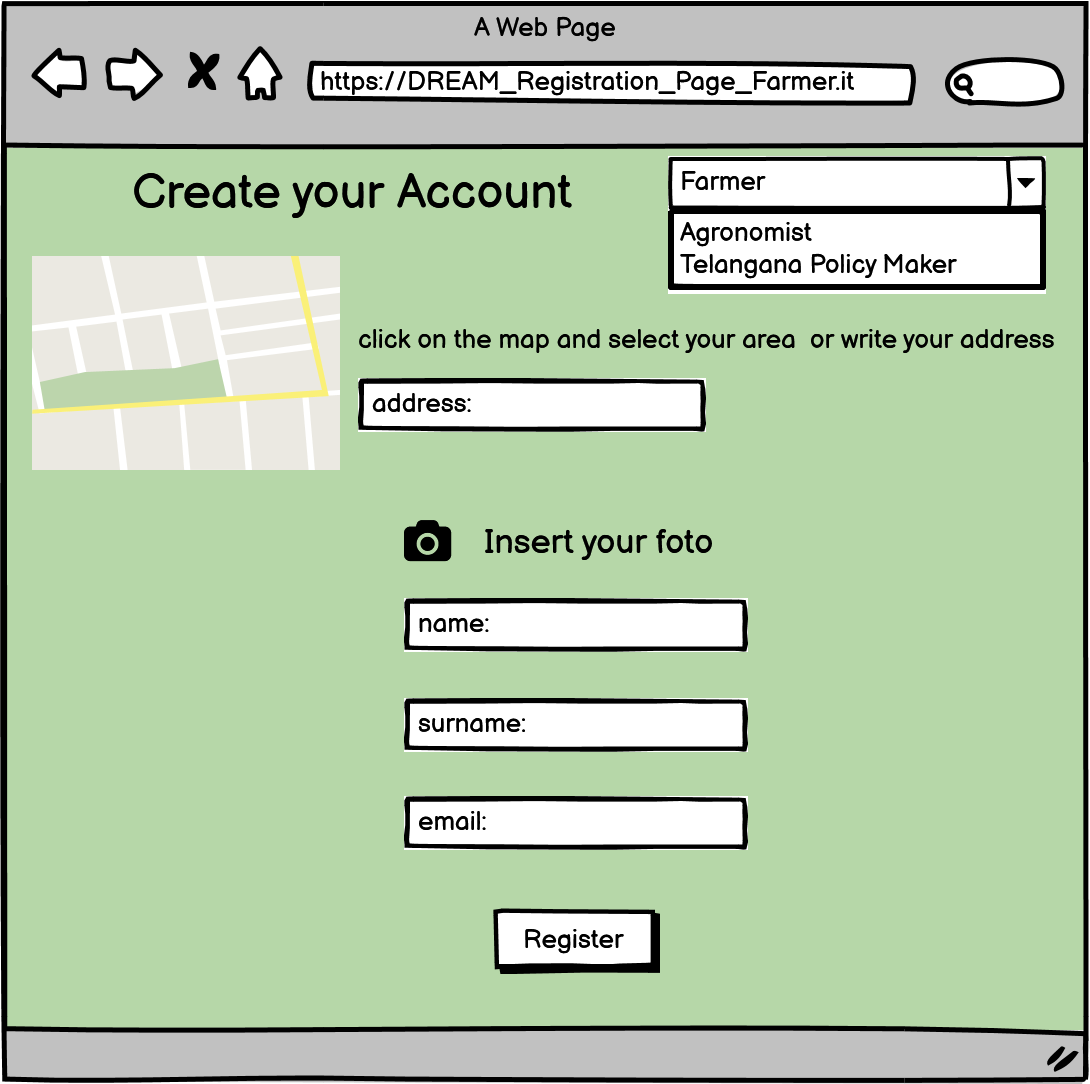
\includegraphics[scale=0.6]{/mockup/1_Registration_Page_Farme.png}
			\caption{Registration Farmer}
		\end{minipage}\hfill
	\end{figure}

	\begin{figure}[ht!]
		\centering
		\begin{minipage}{0.5\textwidth}
			\centering
			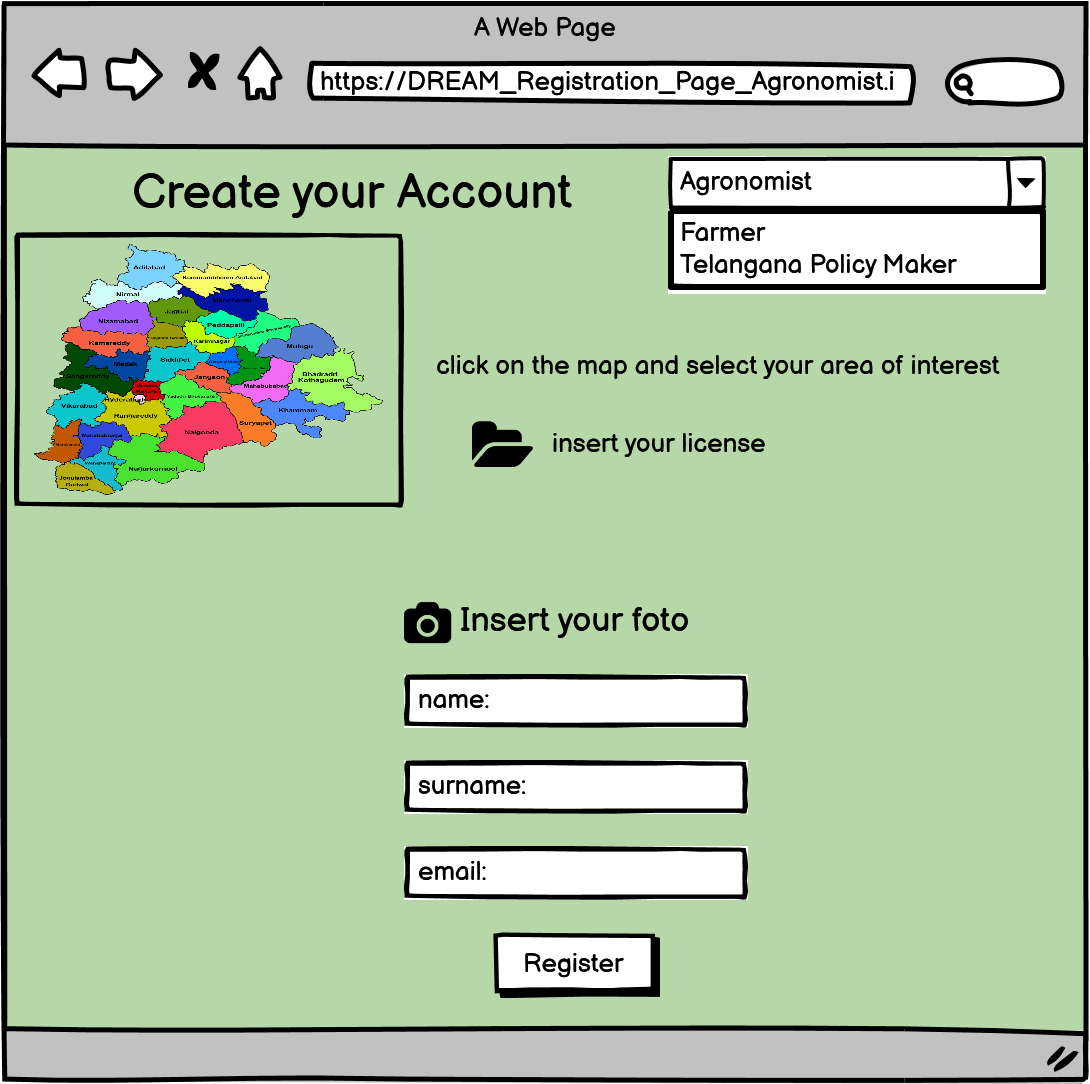
\includegraphics[width=0.95\textwidth]{/mockup/2_Registration_page_Agronomist.png}
			\caption{Registration Agronomist}
		\end{minipage}\hfill
		\begin{minipage}{0.5\textwidth}
			\centering
			\includegraphics[width=0.95\textwidth]{/mockup/3_Registration_Page_TPM.png}
			\caption{Registration TPM}
		\end{minipage}
	\end{figure}

	\begin{figure}[ht!]
		\centering
		\begin{minipage}{0.6\textwidth}
			\centering
			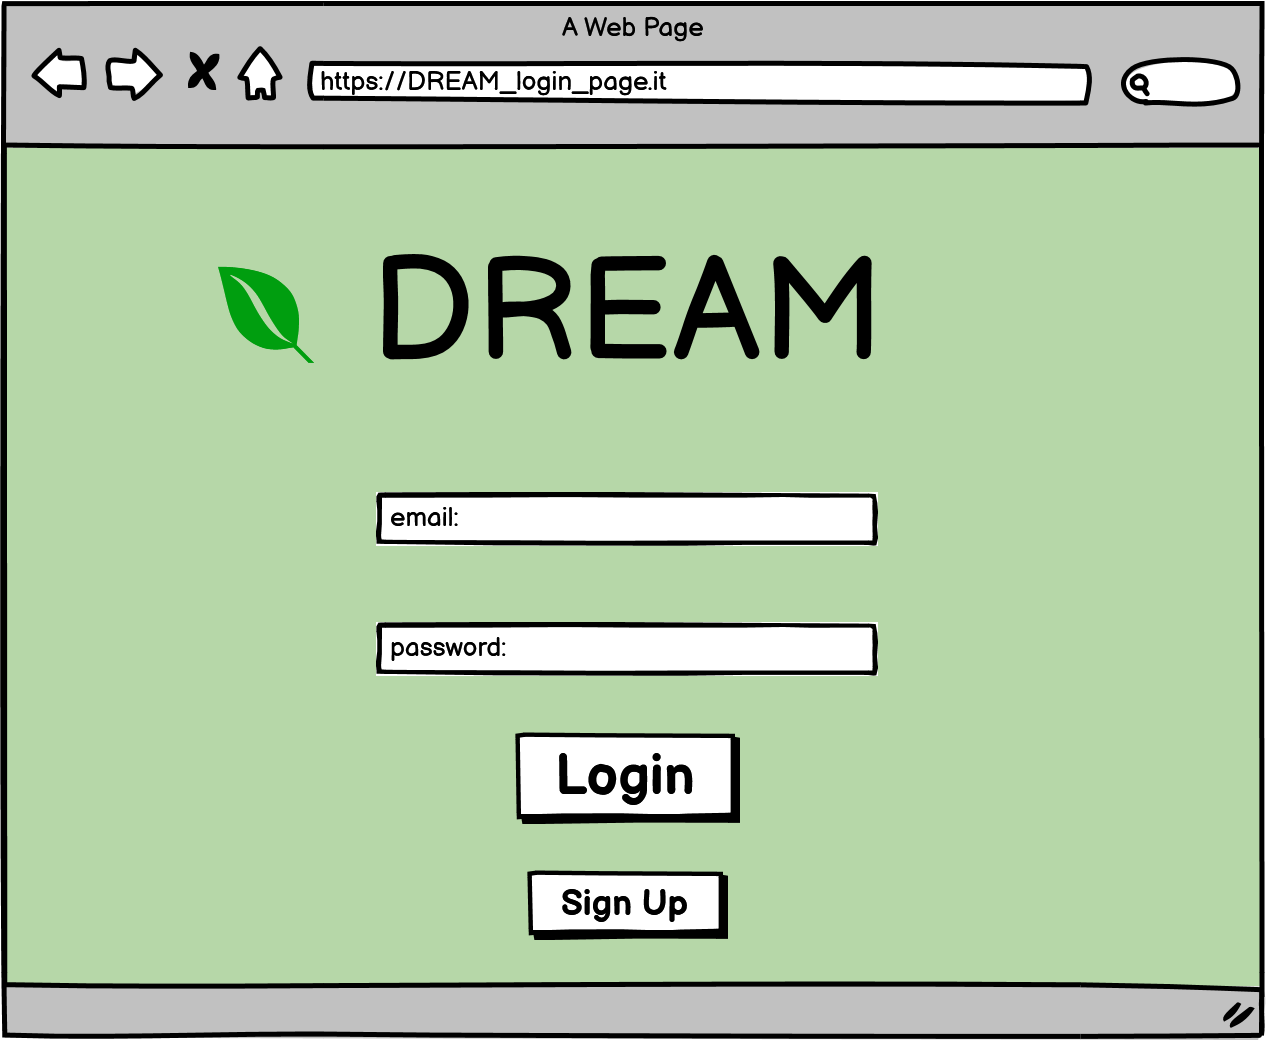
\includegraphics[scale=0.5]{/mockup/4_Login.png}
			\caption{Login Page}
		\end{minipage}
	\end{figure}

	\begin{figure}[ht!]
		\centering
		\begin{minipage}{0.5\textwidth}
			\centering
			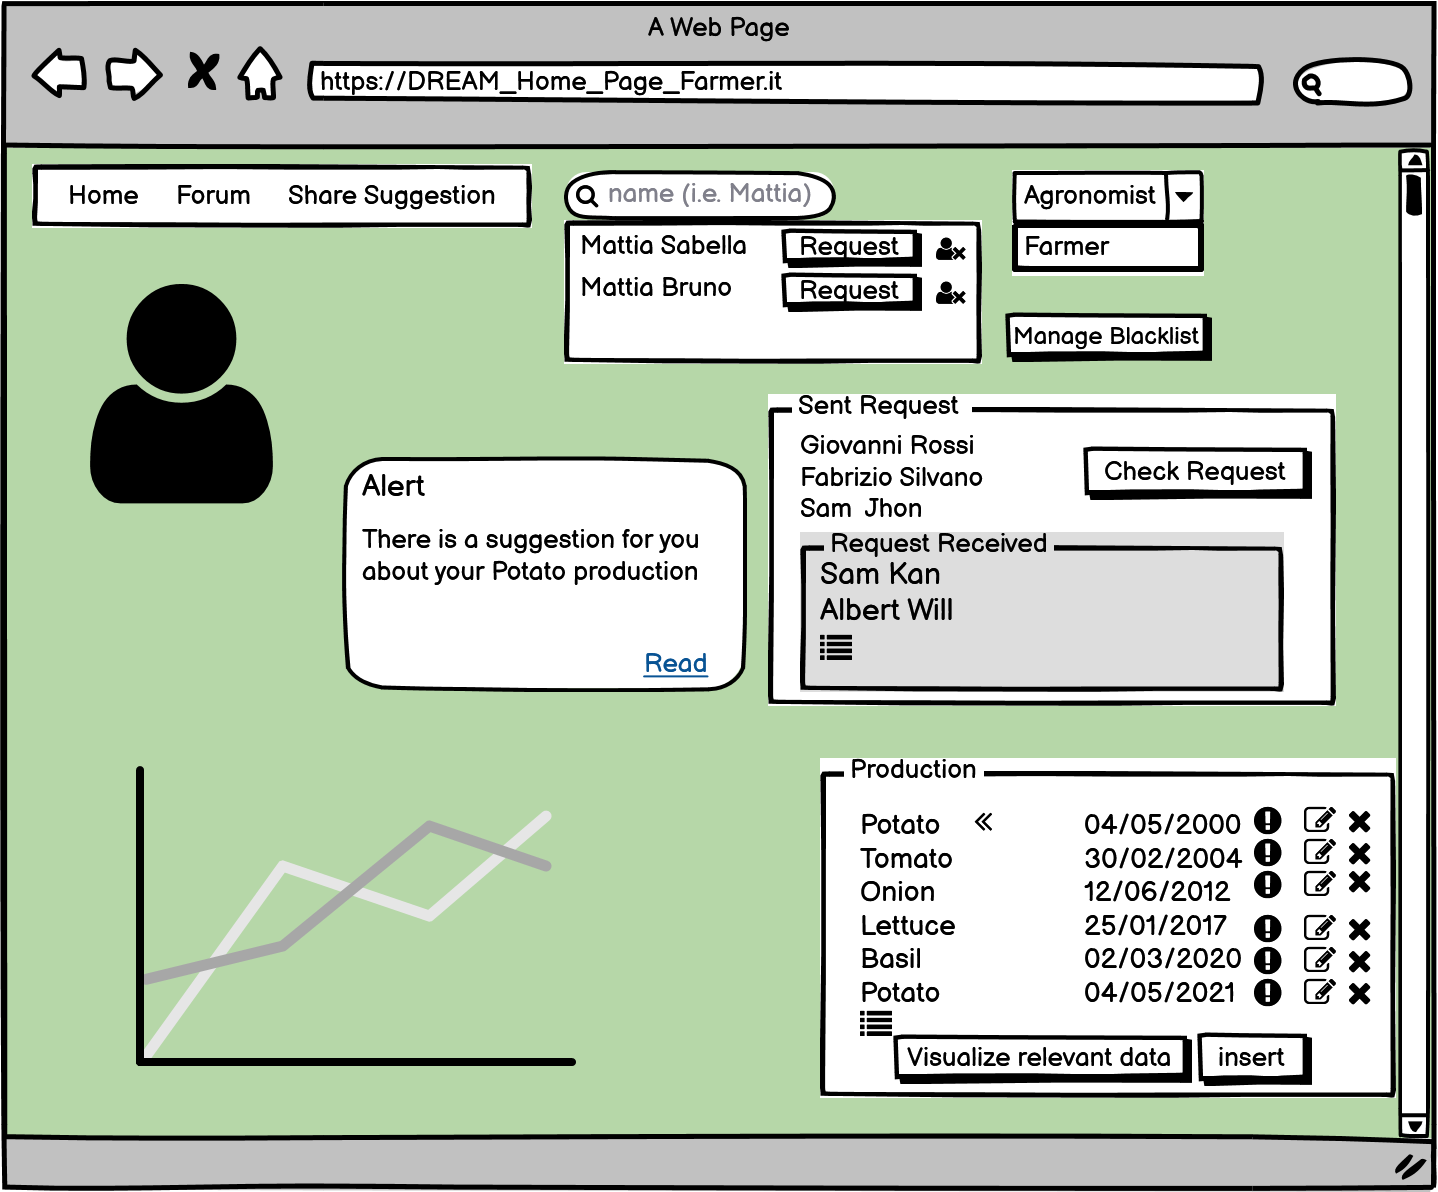
\includegraphics[width=0.95\textwidth]{/mockup/5_Home_page_Farmer.png}
			\caption{Home Page Farmer}
		\end{minipage}\hfill
		\begin{minipage}{0.5\textwidth}
			\centering
			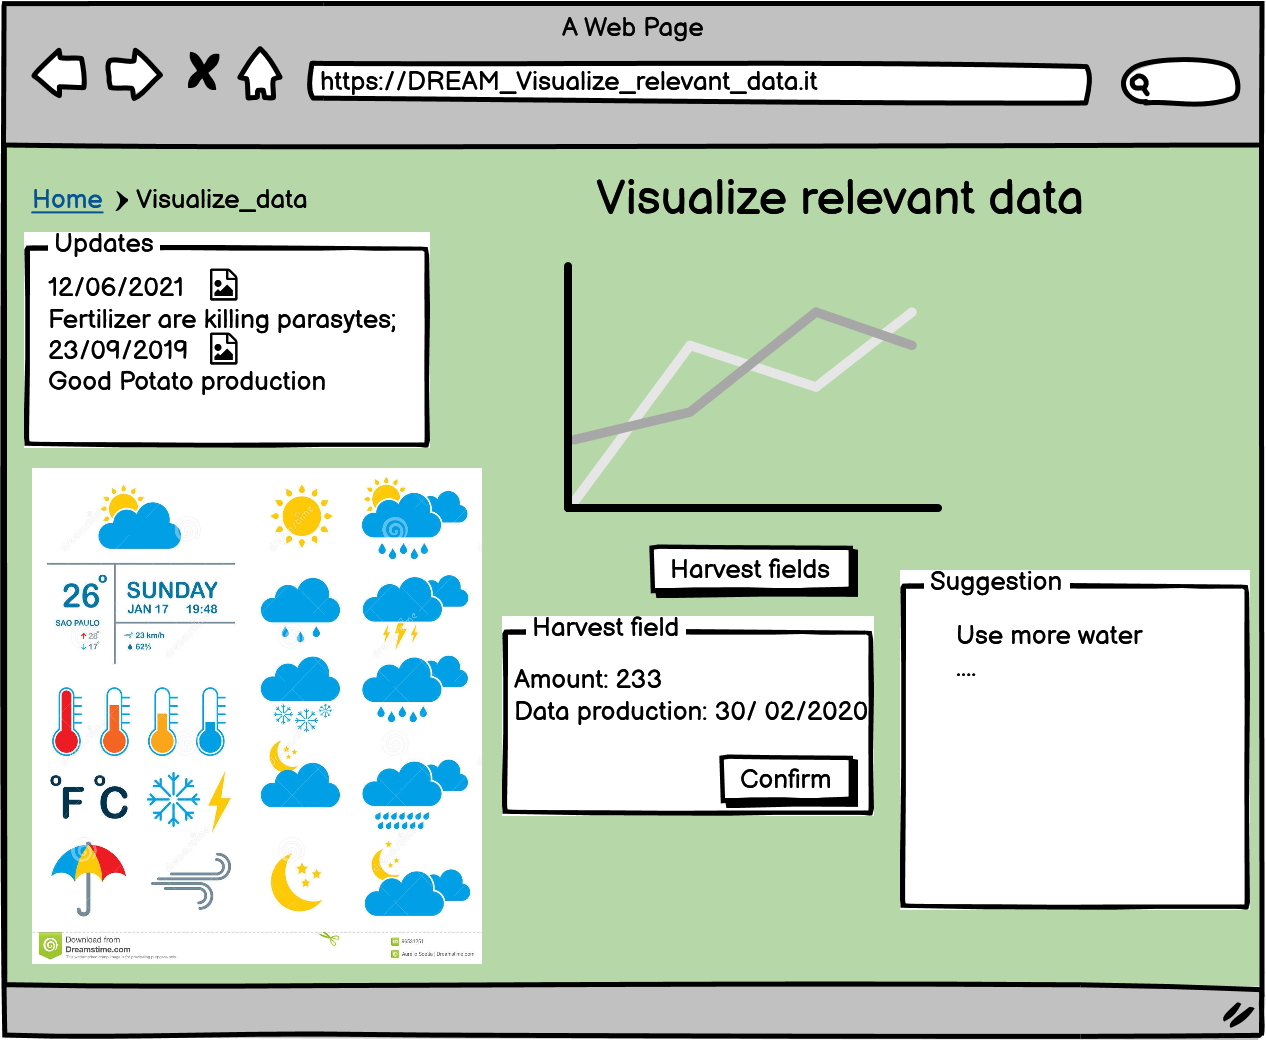
\includegraphics[width=0.95\textwidth]{/mockup/6_Visualize relevant data.png}
			\caption{Farmer Production Field Page}
		\end{minipage}
	\end{figure}

	\begin{figure}[ht!]
		\centering
		\begin{minipage}{0.75\textwidth}
			\centering
			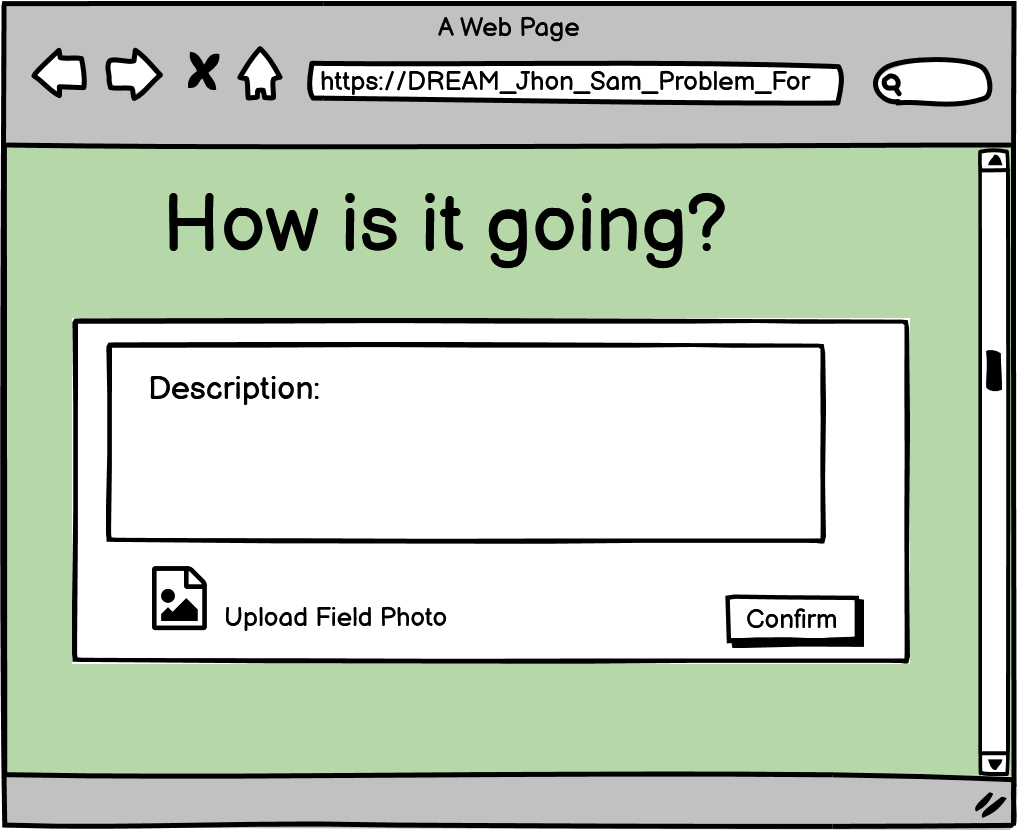
\includegraphics[scale=0.6]{/mockup/9_How is it going_.png}
			\caption{Updates page}
		\end{minipage} 
	\end{figure}


	\begin{figure}[ht!]
		\centering
		\begin{minipage}{0.5\textwidth}
			\centering
			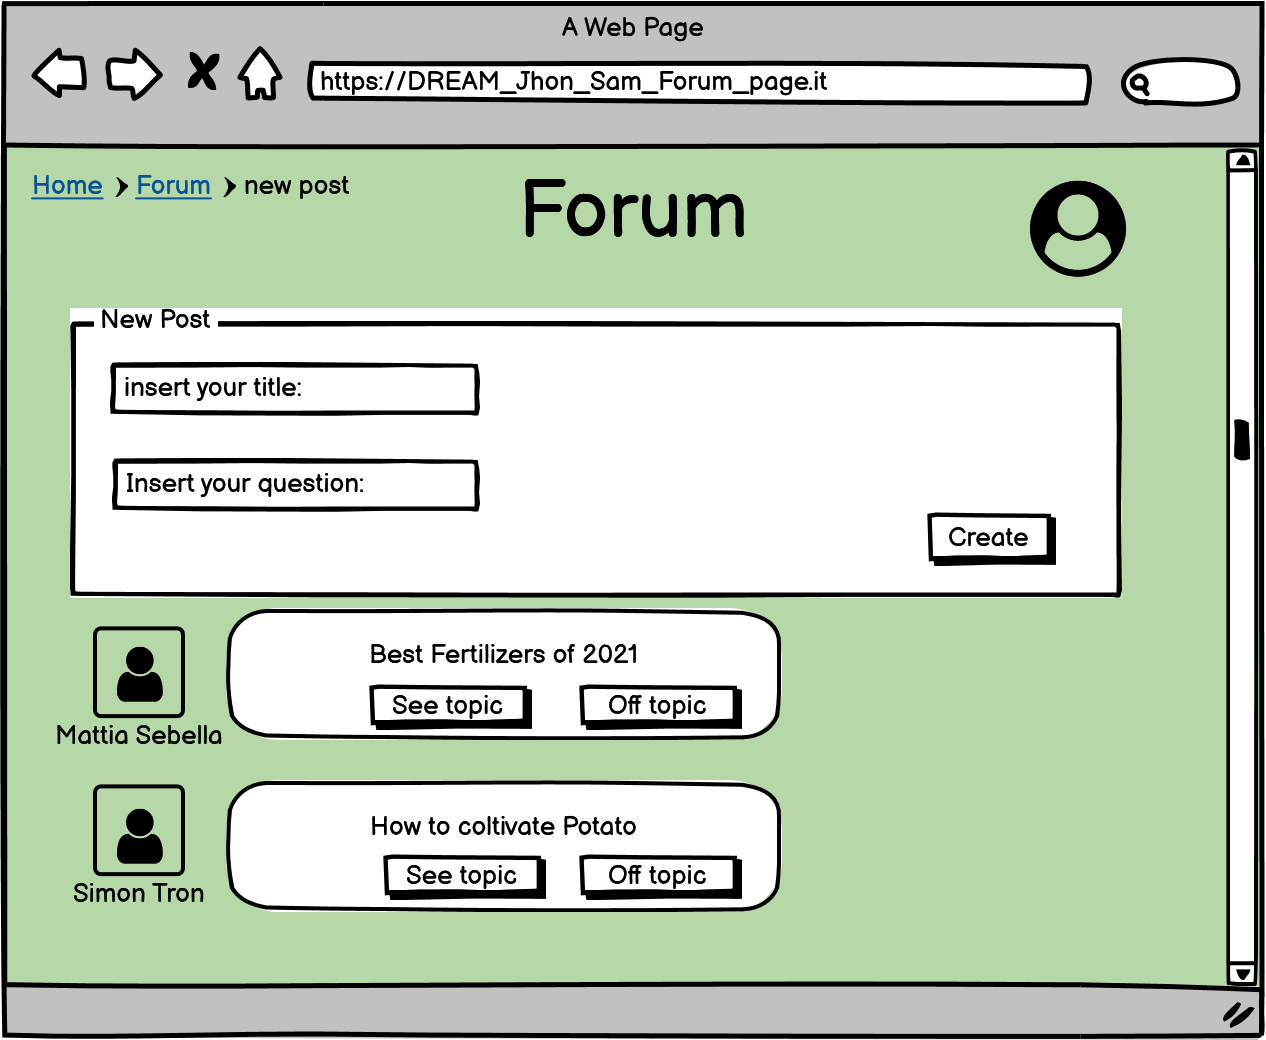
\includegraphics[width=0.95\textwidth]{/mockup/7_Forum.png}
			\caption{Forum Page}
		\end{minipage}\hfill
		\begin{minipage}{0.5\textwidth}
			\centering
			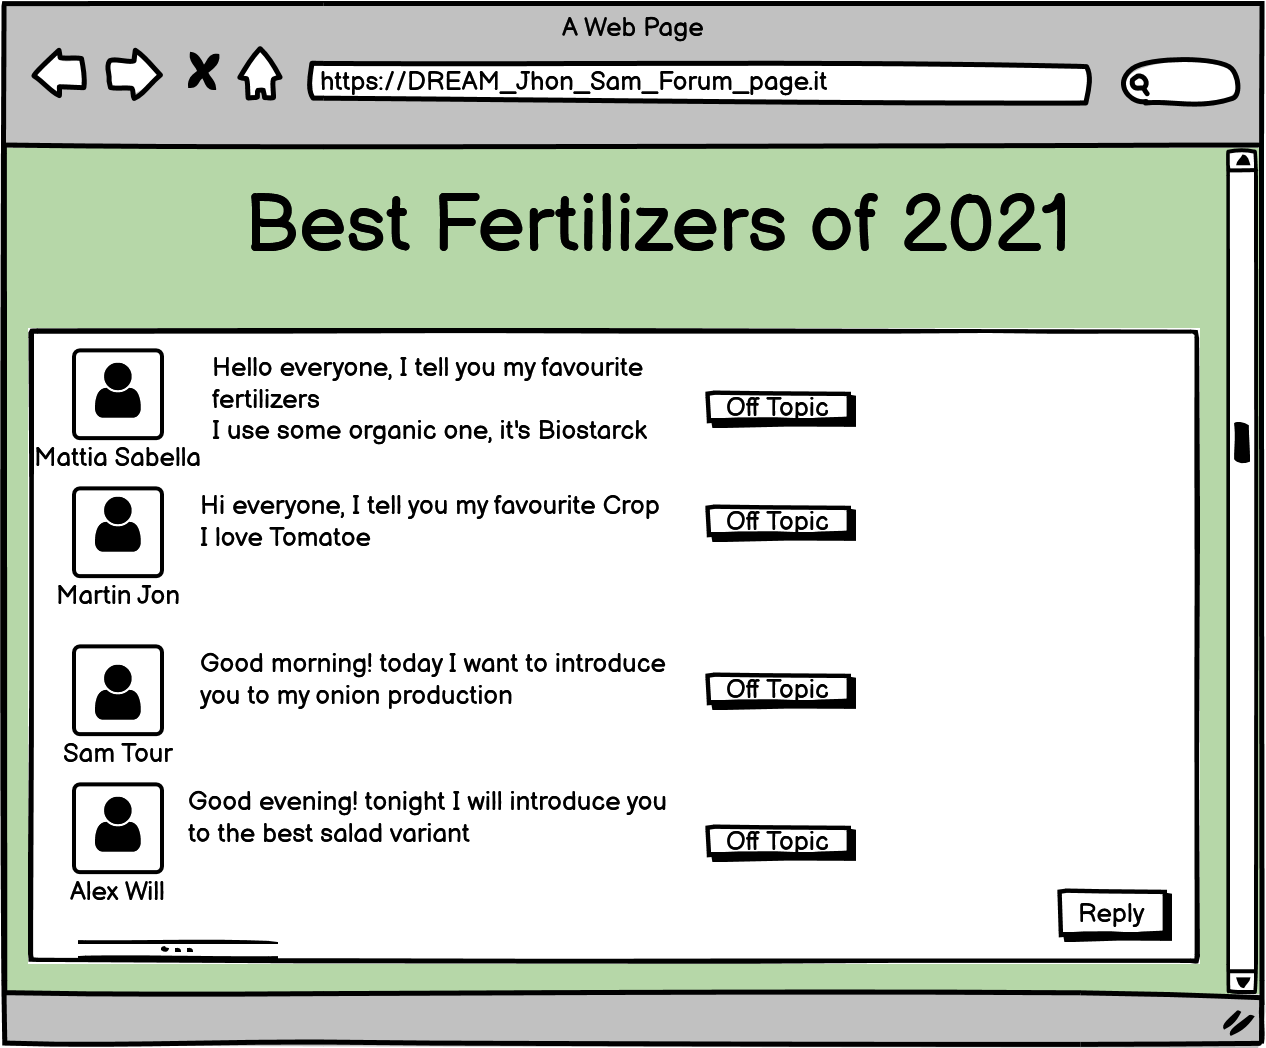
\includegraphics[width=0.95\textwidth]{/mockup/8_Discussion_Forum.png}
			\caption{Topic Page}
		\end{minipage}
	\end{figure}

    \begin{figure}[ht!]
    	\centering
    	\begin{minipage}{0.5\textwidth}
    		\centering
    		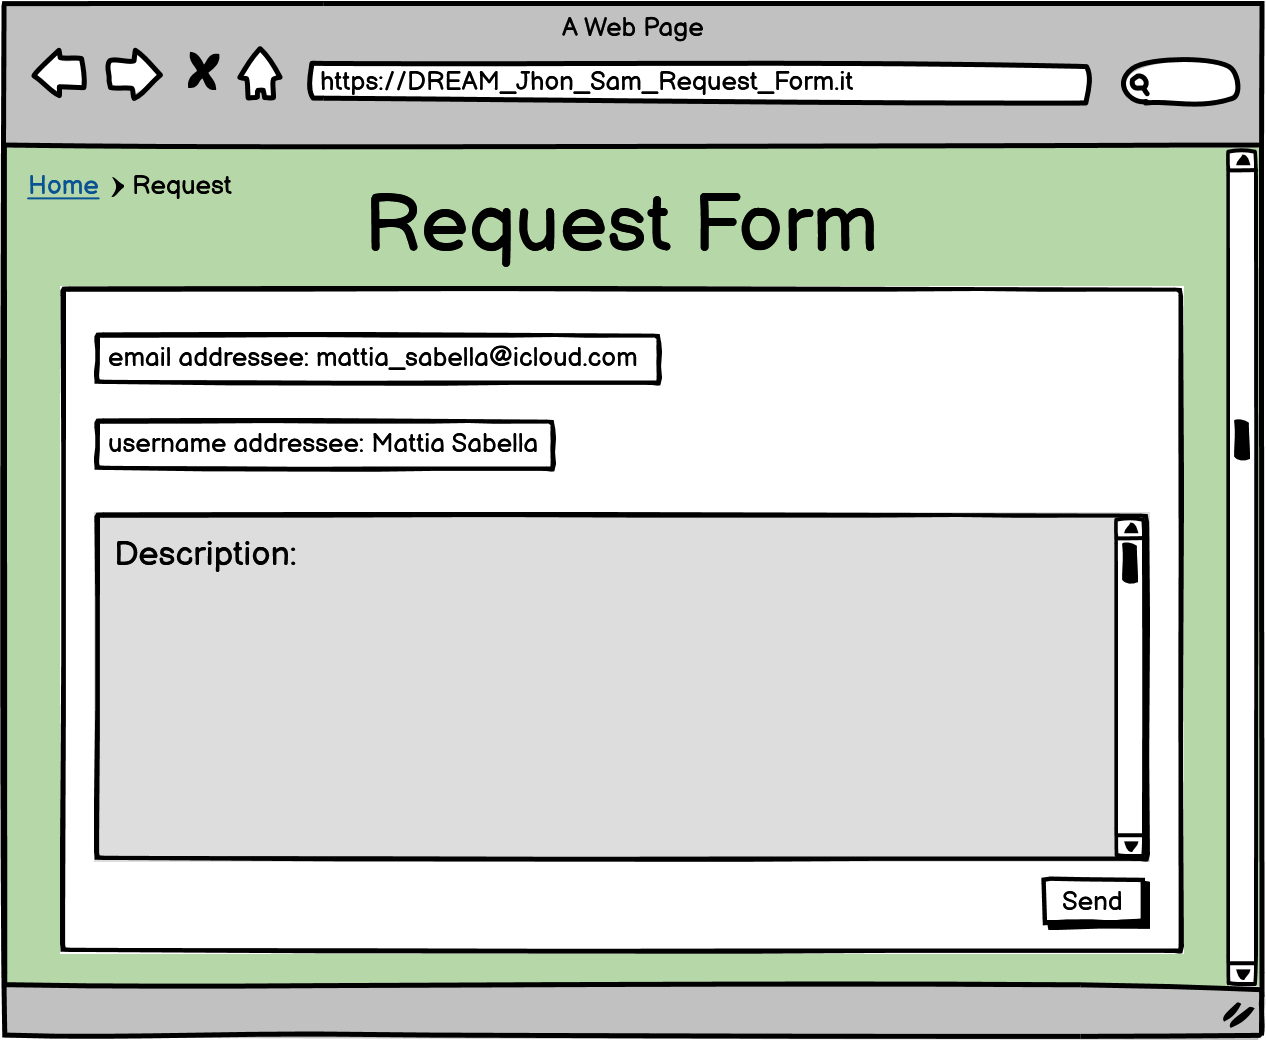
\includegraphics[width=0.95\textwidth]{/mockup/10_Request_Form.png}
    		\caption{Request Form Page}
    	\end{minipage}\hfill
    	\begin{minipage}{0.5\textwidth}
    		\centering
    		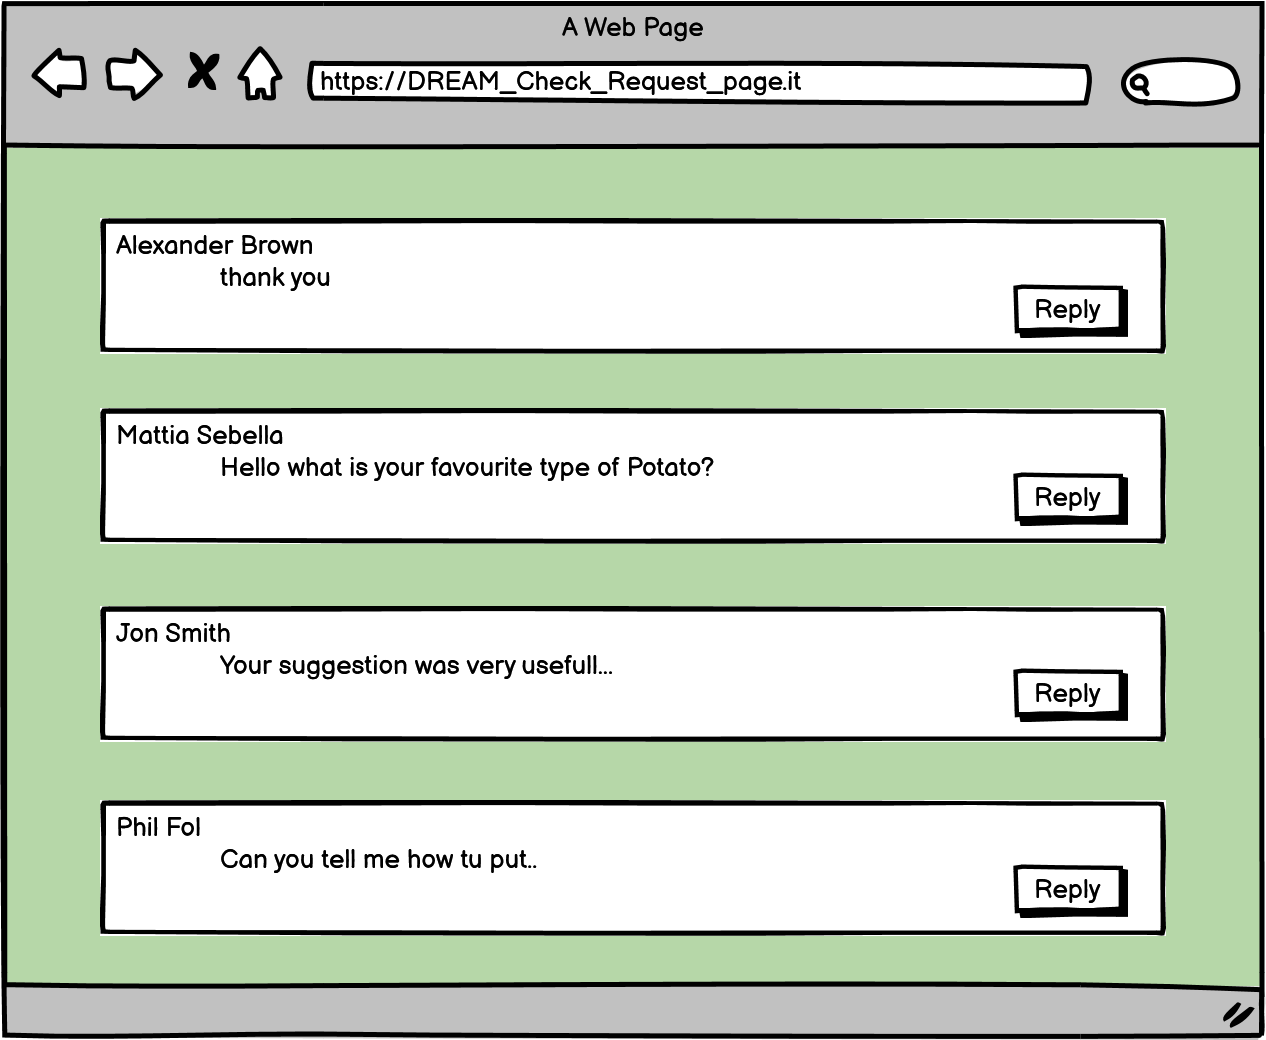
\includegraphics[width=0.95\textwidth]{/mockup/12_Check Request.png}
    		\caption{Requests List Pge}
    	\end{minipage}
    \end{figure}

    \begin{figure}[ht!]
    	\centering
    	\begin{minipage}{0.75\textwidth}
    		\centering
    		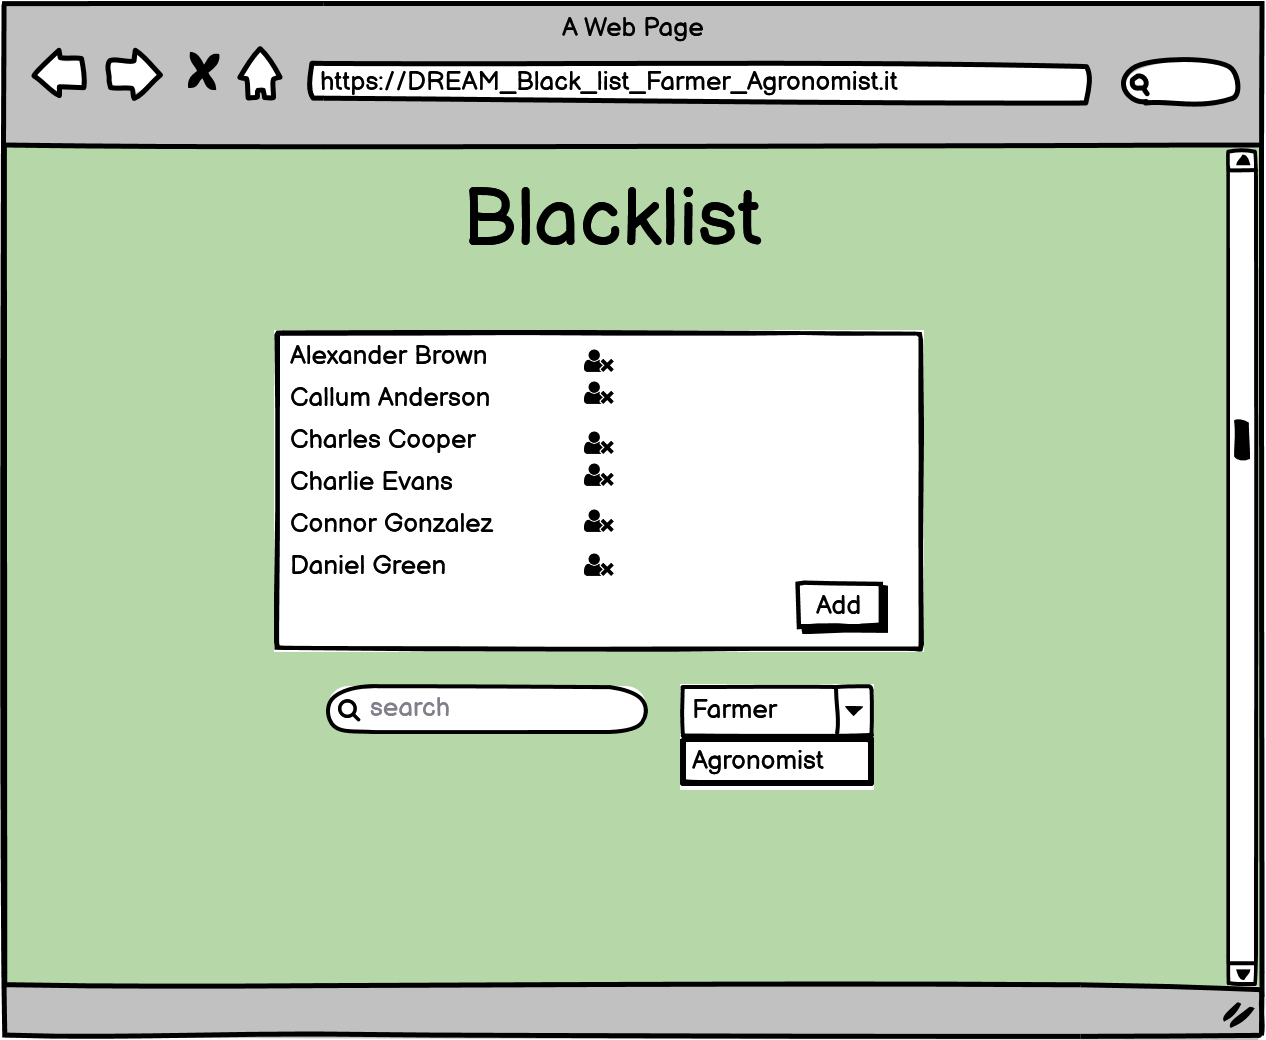
\includegraphics[scale=0.5]{/mockup/11_Blacklist.png}
    		\caption{Blacklist page}
    	\end{minipage} 
    \end{figure}

    \begin{figure}[ht!]
    	\centering
    	\begin{minipage}{0.5\textwidth}
    		\centering
    		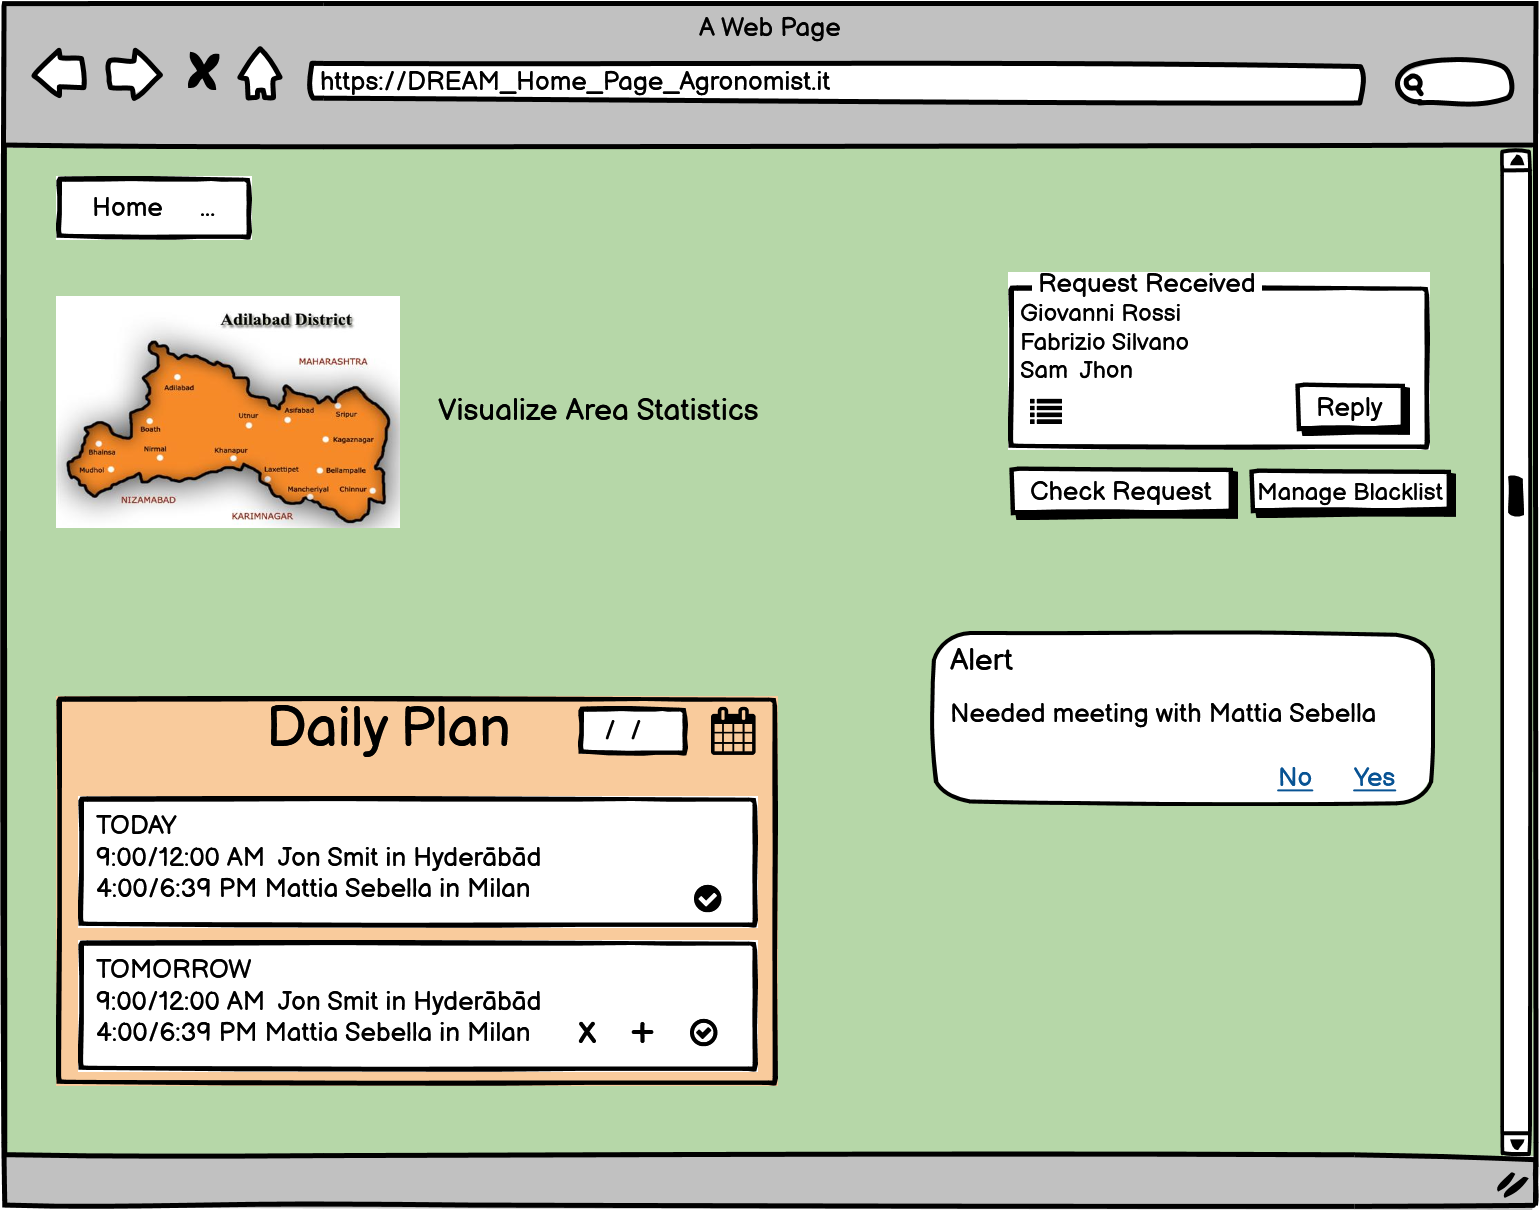
\includegraphics[width=0.95\textwidth]{/mockup/14_Home_Page_Agronomist.png}
    		\caption{Agronomist Home Page}
    	\end{minipage}\hfill
    	\begin{minipage}{0.5\textwidth}
    		\centering
    		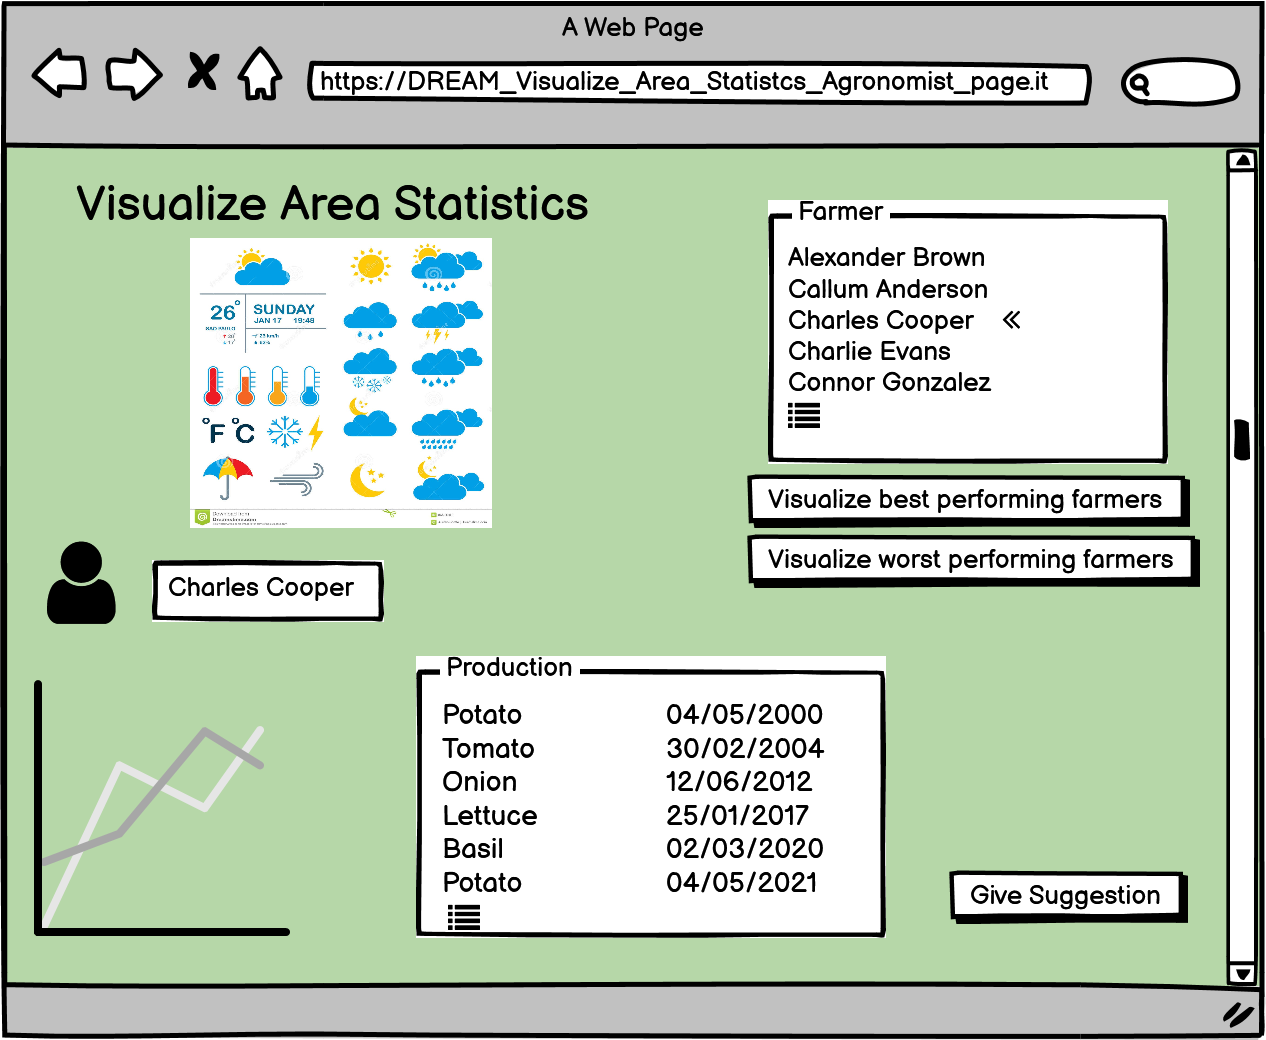
\includegraphics[width=0.95\textwidth]{/mockup/16_Visualize_Area_Agronomist.png}
    		\caption{Statistics Agronomist Page}
    	\end{minipage}
    \end{figure}

    \begin{figure}[ht!]
    	\centering
    	\begin{minipage}{0.75\textwidth}
    		\centering
    		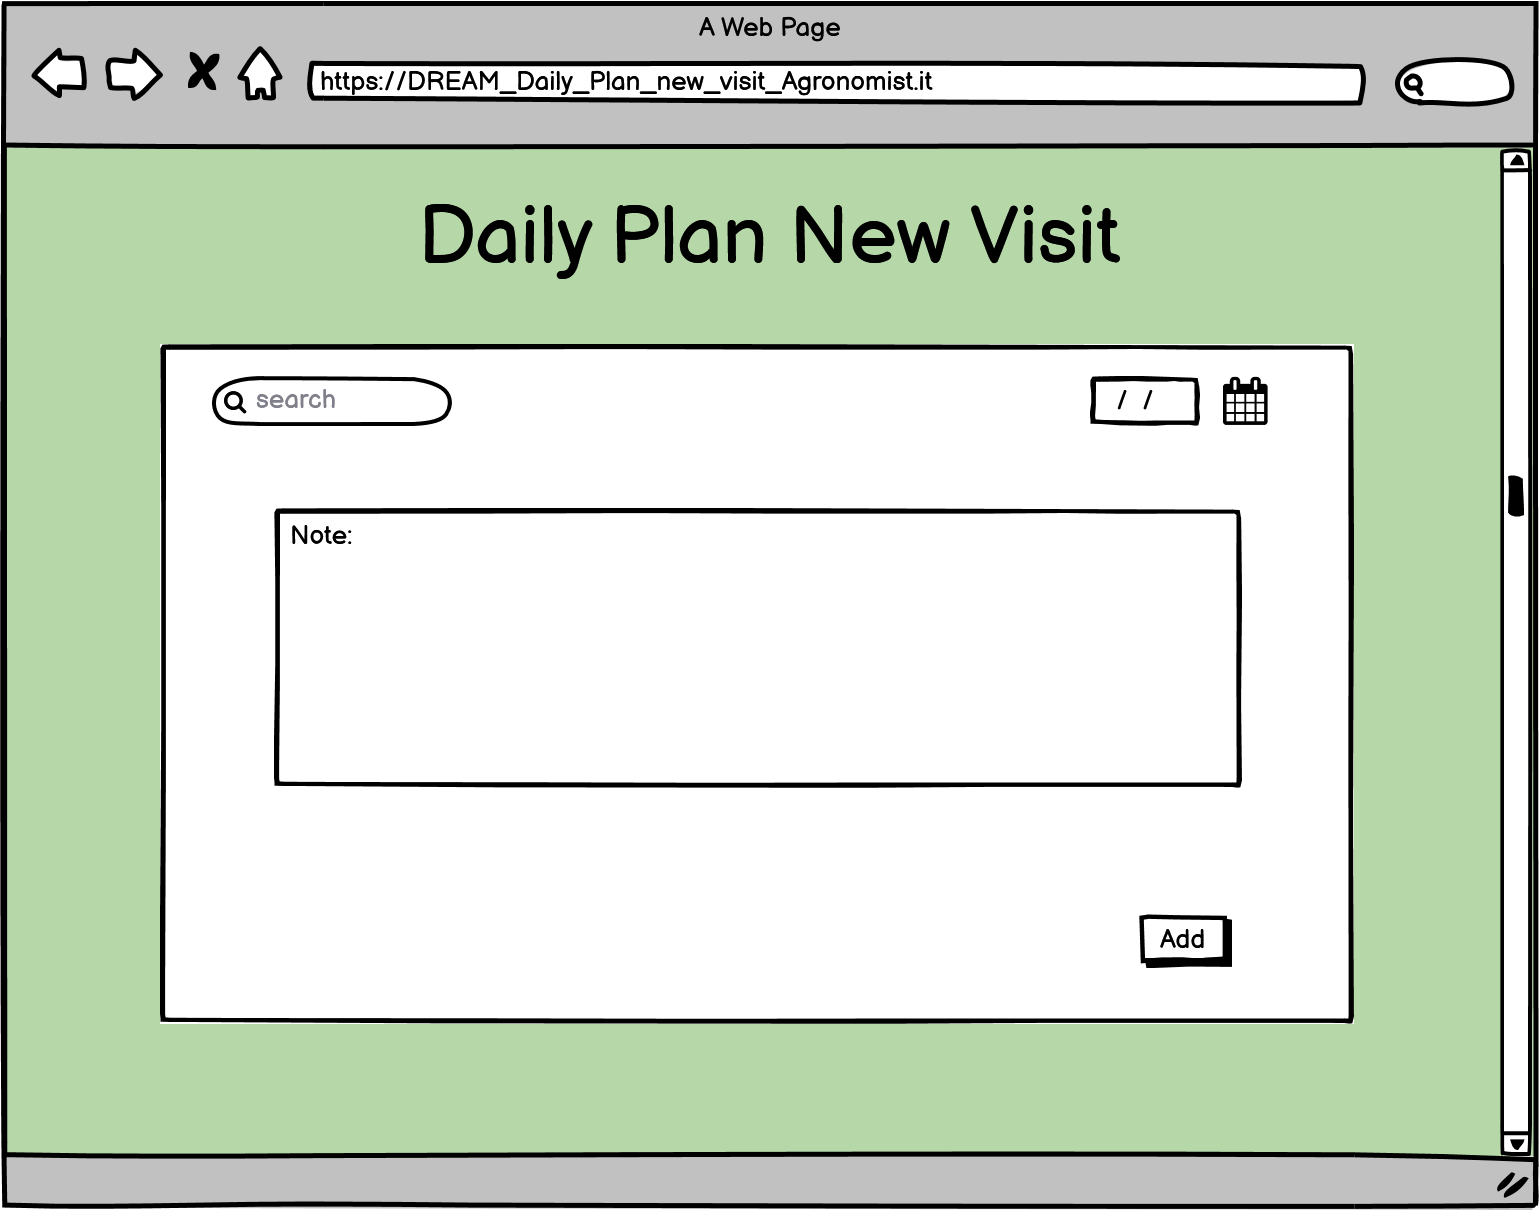
\includegraphics[scale=0.4]{/mockup/15_Daily Plan New Visit.png}
    		\caption{Daily Plan page}
    	\end{minipage} 
    \end{figure}

    \begin{figure}[ht!]
    	\centering
    	\begin{minipage}{0.75\textwidth}
    		\centering
    		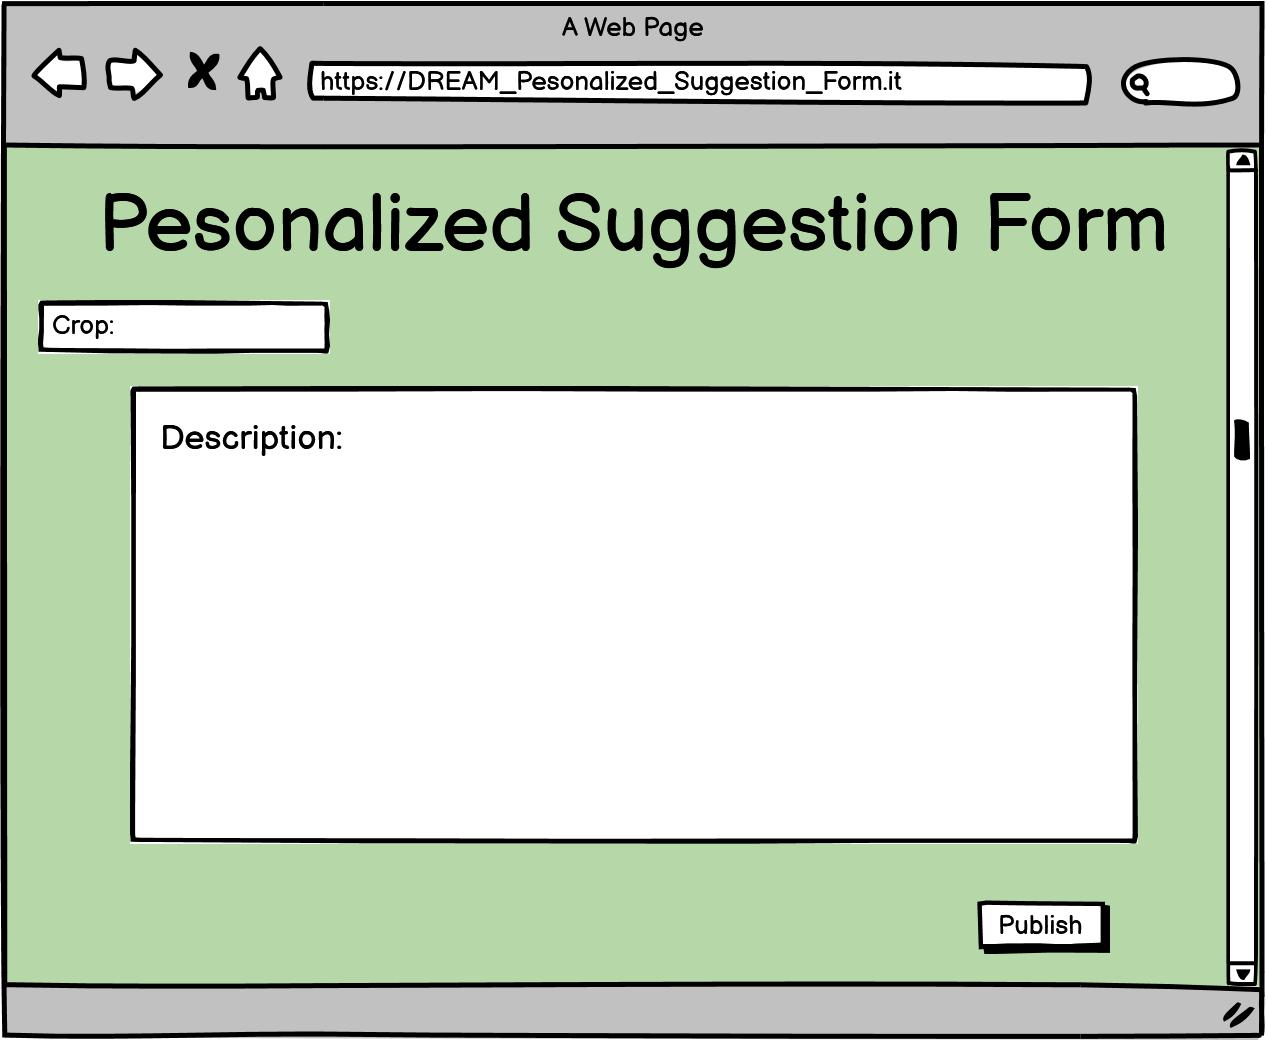
\includegraphics[scale=0.5]{/mockup/13_Suggestion Form.png}
    		\caption{Suggestion Form page}
    	\end{minipage} 
    \end{figure}

    \begin{figure}[ht!]
    	\centering
    	\begin{minipage}{0.75\textwidth}
    		\centering
    		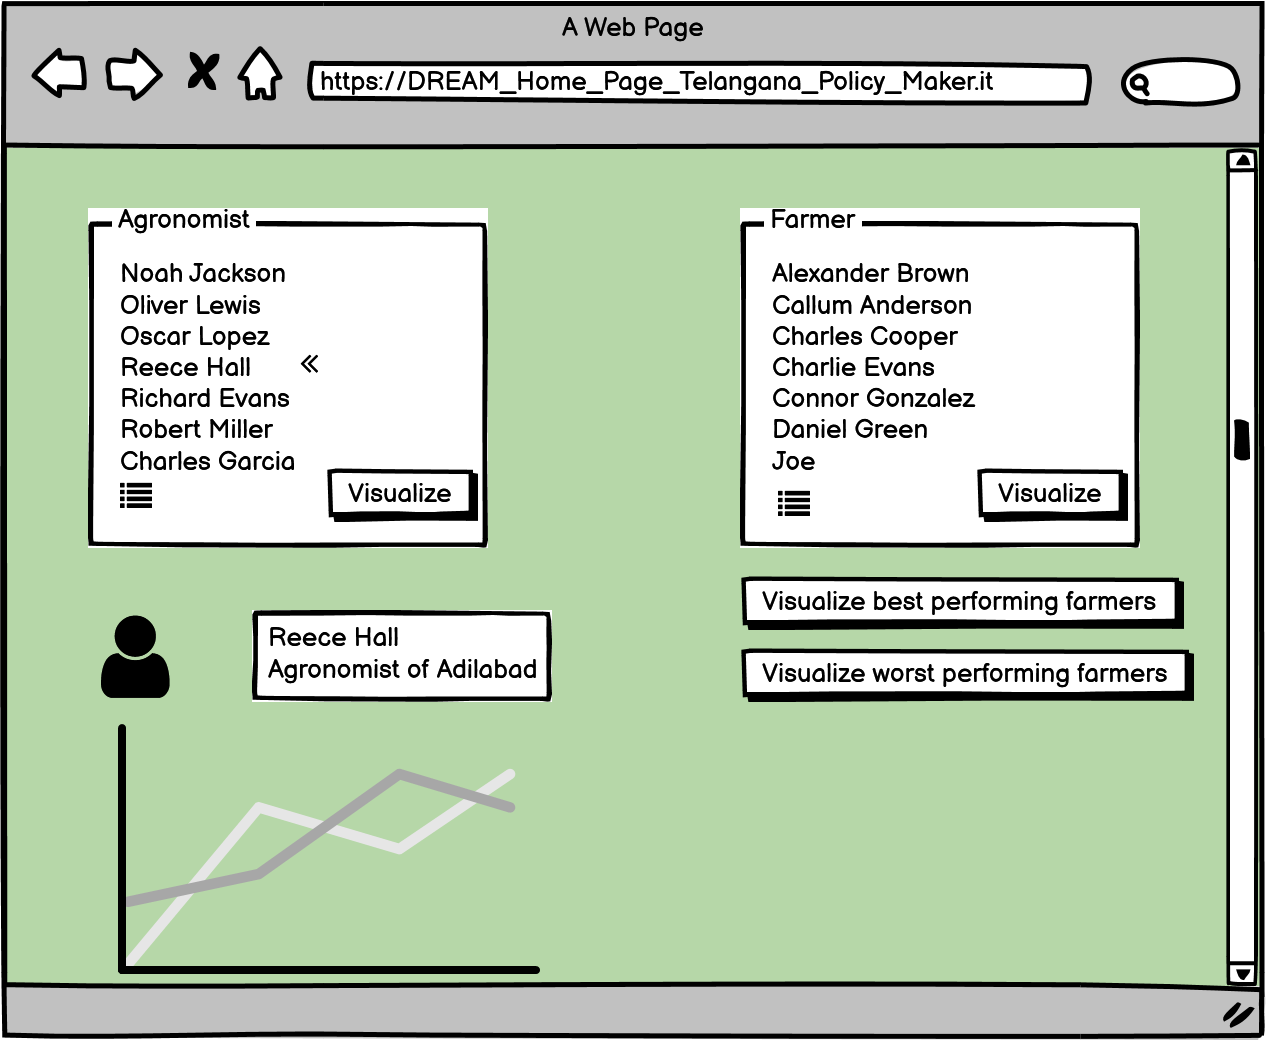
\includegraphics[scale=0.5]{/mockup/17_Home_Page_TPM.png}
    		\caption{TPM Home Page}
    	\end{minipage} 
    \end{figure}
    
	\FloatBarrier
	
	\subsubsection[Hardware Interfaces]{\hyperlink{toc}{Hardware Interfaces}}
	Hardware interfaces to consider are the sensors that must send all the information (eg meteorological info) useful for their production to the farmers. Furthermore a camera useful for Farmers to take pictures of their production to share with the agronomists, to show the progress of their production. 
		
	\subsubsection[Software Interfaces]{\hyperlink{toc}{Software Interfaces}}
	The interfaces used by DREAM is an update browser and MySql. We will need to manage all the information with different logical models in order to store the different kind of data that the application has to deal with.
		
	\subsubsection[Communication Interfaces]{\hyperlink{toc}{Communication Interfaces}}
	Important communications interface to be considered is that system must allow Telangana Policy Maker, Farmer and Agronomist to visualize/insert data, so we weed a communication standards such as HTTP, and FTP to upload license of Agronomist or Telangana Policy Maker, and the pictures uploaded by the Farmer. Moreover Farmer can talk to the Agronomist or to other Farmer, so all messages will be encrypted with an asymmetric key.
		
	\newpage

\subsection[Functional Requirements]{\hyperlink{toc}{Functional Requirements}}
	\label{sec:functionalRequirements}
	This subsection aims to give a \emph{complete} description of the \emph{functional requirements} of our system by defining them together with the domain assumptions that satisfy the identified \textbf{goals}.
	
	\subsubsection[Requirements]{\hyperlink{toc}{Requirements}}
		\begin{enumerate}[label=\textbf{R\arabic*}]
			\item \label{req:R1} Users must be authenticated as Farmer, or Agronomist, or Telengana's Policy Maker.
			\item \label{req:R2} Farmer, Agronomists and Telengana's Policy Makers register  to the application through mandatory fields.
			\item \label{req:R3} In phase of registration, Farmers must specify one and only one geographical area of working.
			\item \label{req:R4} Agronomists and Telengana's Policy Makers who registered inserted in the application their valid license.
			\item \label{req:R5} Agronomist must specify in the system at least one area of interest.
			\item \label{req:R6} Agronomists will access farmer's data and statistics only from that ones in their area of interest.
			\item \label{req:R7} Private requests between a farmer and an agronomist can't be accessed by other users.
			\item \label{req:R8} Suggestions related to a particular crop field can be accessed by every farmer who owns that crop field.
			\item \label{req:R9} Private suggestions coming from an Agronomist can be accessed only by the Farmer who received them.
			\item \label{req:R10} Agronomists can access to the list of request from farmers.
			\item \label{req:R11} Agronomists can reply to farmer's request through a chat window.
			\item \label{req:R12} The system must keep track of how many times a farm has been visited.
			\item \label{req:R13} Monthly the system notifies the agronomist with the list of farms which has not been visited at least twice.
			\item \label{req:R14} The system must allow the Agronomist to keep updated his daily plan.
			\item \label{req:R15} After a proper time window, the daily plan declared by an Agronomist becomes fixed and immutable.
			\item \label{req:R16} Topics in discussion forums must be initialized by a farmer.
			\item \label{req:R17} The system allows farmers to access public discussions.
			\item \label{req:R18} Off-Topic discussions can be reported by farmers to be deleted.
			\item \label{req:R19} When a topic is reported a certain number of times, the topic will be deleted.
			\item \label{req:R20} The system allows agronomists to block spam requests by farmers by including them in a blacklist.
			\item \label{req:R21} The system allows farmers to insert production data through mandatory fields of a form.
			\item \label{req:R22} Farmers can visualize statistics about their production data built by the system.
			\item \label{req:R23} Statistics build over farmer's production, performance etc are based on three parameters: amount of crop harvested, amount of crop planted, weather conditions.
			\item \label{req:R24} The system allows farmers to search agronomists/farmers they want to contact.
			\item \label{req:R25} Farmers can send requests directly to agronomists and other farmers.
			\item \label{req:R26} Farmers visualize Agronomists' replies in an inbox window.
			\item \label{req:R27} Farmers and Agronomists visualize other Farmers requests in an inbox window.
			\item \label{req:R28} Allow Agronomists to visualize weather forecasts in their area of interest.
			\item \label{req:R29} Allow Farmers to visualize weather forecasts in their geographical area.
			\item \label{req:R30} The system classifies best performing farmers based on their performance index.
			\item \label{req:R31} The system allows Telengana Policy Makers to visualize best and worst performing farmers according to their performance indexes.
			\item \label{req:R32} The system allows Telengana's Policy Makers to visualize Agronomists statistics.
			\item \label{req:R33} Farmers can share pictures of their production field through the system.
			\item \label{req:R34} Farmer and Agronomists can manage a blacklist containing contacts of other Farmers.
			\item \label{req:R35} The system allows agronomists and farmers to reply to other farmer's help request.
			\item \label{req:R36} The system allows Agronomist to visualize best and worst performing farmers according to their performance indexes.
		\end{enumerate}
	
	\newpage
	
	\subsubsection[Mapping]{\hyperlink{toc}{Mapping}}
		\label{sec:goalSatisfaction}
		
		
			\begin{longtable}{p{0.26\linewidth}p{0.75\linewidth}}
				\toprule
				\textbf{Goal} & G1\\
				\midrule
				\textbf{Domains} & DA1, DA2, DA5, DA6, DA7, DA16, DA17, DA18, DA19, DA20, DA21, DA22\\
				\midrule
				\textbf{Requirments} & R1, R2, R3, R21, R22, R23, R29, R33 \\
				\bottomrule
				\caption{\emph{G1 Mapping}}
			\end{longtable}

			\begin{longtable}{p{0.26\linewidth}p{0.75\linewidth}}
				\toprule
				\textbf{Goal} & G2\\
				\midrule
				\textbf{Domains} & DA5,DA18, DA19,DA22\\
				\midrule
				\textbf{Requirments} & R1, R2, R3, R21, R33 \\
				\bottomrule
				\caption{\emph{G2 Mapping}}
			\end{longtable}
		
			\begin{longtable}{p{0.26\linewidth}p{0.75\linewidth}}
				\toprule
				\textbf{Goal} & G3\\
				\midrule
				\textbf{Domains} & DA8, DA12, DA13, DA18, DA19\\
				\midrule
				\textbf{Requirments} & R1, R2, R8, R16, R17, R18, R19, R24, R25, R27, R34, R35 \\
				\bottomrule
				\caption{\emph{G3 Mapping}}
			\end{longtable}		
		
			\begin{longtable}{p{0.26\linewidth}p{0.75\linewidth}}
				\toprule
				\textbf{Goal} & G4\\
				\midrule
				\textbf{Domains} & DA3, DA4, DA8, DA11, DA12, DA13, DA14, DA19\\
				\midrule
				\textbf{Requirments} & R1,R2, R4, R7, R9, R10, R20, R24, R25, R27, R34, R35 \\
				\bottomrule
				\caption{\emph{G4 Mapping}}
			\end{longtable}		
		
			\begin{longtable}{p{0.26\linewidth}p{0.75\linewidth}}
				\toprule
				\textbf{Goal} & G5\\
				\midrule
				\textbf{Domains} & DA1, DA2, DA3, DA4, DA9,DA10, DA11,DA14, DA15, DA19\\
				\midrule
				\textbf{Requirments} & R1,R2, R4,R5,R6, R12, R13, R14, R15, R28 \\
				\bottomrule
				\caption{\emph{G5 Mapping}}
			\end{longtable}	
		
			\begin{longtable}{p{0.26\linewidth}p{0.75\linewidth}}
				\toprule
				\textbf{Goal} & G6\\
				\midrule
				\textbf{Domains} & DA1, DA2, DA5, DA14, DA15, DA19\\
				\midrule
				\textbf{Requirments} & R1, R2, R5, R6, R21, R22, R23, R28, R30, R36 \\
				\bottomrule
				\caption{\emph{G6 Mapping}}
			\end{longtable}
		
			\begin{longtable}{p{0.26\linewidth}p{0.75\linewidth}}
				\toprule
				\textbf{Goal} & G7\\
				\midrule
				\textbf{Domains} & DA1, DA5, DA14, DA19\\
				\midrule
				\textbf{Requirments} & R1, R2, R3, R4, R21, R22, R23, R30, R31 \\
				\bottomrule
				\caption{\emph{G7 Mapping}}
			\end{longtable}
		
			\begin{longtable}{p{0.26\linewidth}p{0.75\linewidth}}
				\toprule
				\textbf{Goal} & G8\\
				\midrule
				\textbf{Domains} & DA2, DA3, DA4, DA11, DA14, DA15, DA19\\
				\midrule
				\textbf{Requirments} & R1, R2, R4, R5, R12, R30, R32 \\
				\bottomrule
				\caption{\emph{G8 Mapping}}
			\end{longtable}						
		\newpage

\subsection[Use Cases Identification]{\hyperlink{toc}{Use Cases Identification}}
	In the following subsection the usage of the system is going to be described first with a general description using scenarios and then in a more specific way using use case diagrams.
	
	\subsubsection[Scenarios]{\hyperlink{toc}{Scenarios}}
		Consider these scenarios in order to clarify the usage of the system and the further description with use case diagrams.
		
		\begin{enumerate}[label=\textbf{SCENARIO \arabic*}]
			\item \label{sce:sce1} FARMER MANAGES HIS FIELDS \\ 
			Odoacre is a newbie farmer, and he owns so many lands (one of them is full of potatoes) that he does not know how to properly manage them. Odoacre discovered DREAM, a service that can help him to achieve his goal of improving, then after registration he puts in the system data about his production fields. For each declared field Odoacre waits 2 seconds (or less...)
			until the system calculates for him statistics about weather forecasts of his geographical location of his lands.
			Odoacre now has more knowledge on how to plan his production for the next week according to weather forecats, but still
			he is a newbie and wants to know something else and more specific about his type of production, furthermore, he faces a problem: his potato land does not grow properly because of parasytes.
			Odoacre notices that he can actually declare his problem in the system and upload a photo of his field; it does so, and he hopes that someone some day visualizes what he uploaded and then helps him.
			The next day Odoacre opens again DREAM and sees personalized suggestions coming from experienced farmers and agronomists about his potato land, which kind of fertilizers and pesticides he should use and even which kind of crops he should plant.
			Odoacre "harvests" theese golden information and puts in practice what he learned, and sooner or later he will notice an improvement on his production. Indeed, after a month or so, he checks his potato field and notices that finally, twentynine out of thirty potatoes are fully grown and they are ready to be gathered. Orlando then updates DREAM parameters of his production field, and he declares that his monthly production for the potato land is ended, and the field is now empty and ready for the next growth. DREAM stores his declaration, resets all the parameters and immediately updates the performance index of the Farmer according to how many potatoes he harvested and
			how many of them he planted in that month.
			
			\item \label{sce:sce2} FARMER SHARES SUGGESTIONS \\
			Glauco is an experienced farmer who masters the art of agriculture, and he wants to share his knowledge with other farmers. He keeps track of his failures and successes and writes a text full of personalized suggestions useful for manage production fields according to the type of production, the weather etc...
			Since Glauco uses DREAM a lot, he shares information contained in his text through the system, which analyzes it and forwards specific suggestions to specific fields of other farmers in need.
			Odoacre (who now needs help with his carrots land) and Gastone (who faces the same problems of Odoacre) see in their Carrots Field Panel the suggestions of Glauco, since they were forwarded by the system itself.
			
			\item \label{sce:sce3} FARMER COMMUNICATES THROUGH DISCUSSION FORUMS \\ 
			Melchiorre is a farmer who plants crops which are really unpopular. Since 90 percent of experienced farmers does not think that someone would plant uncommon crops (like Achuqcha), no one of them even prepared personalized suggestions about these kind of batch. Melchiorre wants to improve is production of Achuqcha, but he does not see any personalized suggestion about his production field! 
			Melchiorre won't give up, he discovered that DREAM offers the possibility of create discussion forums with other farmers, and thinks that maybe in this way multiple farmers will notice him.
			He creates the discussion forum, writes the first post describing all his needs with the Achuqcha field, and waits for eventual replies. 
			Telemaco, Tebaldo and Teodosio are three farmers that plant Achuqcha since many years, and they use DREAM a lot. They periodically checks the discussion forums present in the system, and they see a topic named "I need help with Achuqcha!" created by Melchiorre. They open it, they read the first post and immediately they formulate and send a reply, each one coming from a different farmer (on different computers...).
			Melchiorre is so anxious that he refreshes the discussion forum page so many times, and finally he notice three useful replies coming from Telemaco, Tebaldo and Teodosio. As expected, multiple farmers which believed to be the only ones in the world that plant Achuqcha replied to him, and helped him with his production field; Melchiorre is now happy and can improve his production.
			
	
			\item \label{sce:sce4} FARMER AND AGRONOMISTS COMMUNICATES THROUGH DIRECT MESSAGES \\ 
			Olivia is a farmer who plants the strange (but delicious) crop of Kiwano. Unlike Melchiorre, Olivia does not want that eventual replies to her requests of help are shared with other Farmers, she is a greedy person, so she avoids
			the use of public discussion forums. Still, Olivia needs help with his production field of Kiwano, as no one has still inserted in the system personalized suggestions about this kind of crop.
			Olivia discovers that DREAM offers the possibility to send direct and private email-like messages to a Farmer or to an Agronomist, so she formulates his request and she send it to two persons, Attilio (a farmer who plants Kiwano too) and Nicodemo (an Agronomist).
			On the other side, Attilio and Nicodemo check their inbox in DREAM and notice the message of Olivia; (individually) they write a reply full of suggestions and they forward it to Olivia.
			Olivia sees the reply on her inbox in DREAM, reads it and finally she can improve her production of Kiwano.
			
			\item \label{sce:sce5} AGRONOMIST VISUALIZES AREA STATISTICS \\ 
			Amilcare is an agronomist whose working area of interest is the district of Adilabad in Telengana. Since Amilcare uses DREAM a lot, he often uses the "Visualize Area Statistics" function of the system to see  weather forecasts of
			his area of interest. He can also see the performance indexes of farmers working on his same geographical area, and he notices that among them Frida is performing particularly well (bad), so he decides to investigate by expanding information about her production fields. Amilcare can now see which crops Frida is planting and how her production is going; he finds out that Frida faced a problem with her field of corn, furthermore he checks the photo she published about her land, so he thinks that her field of strawberries can be improved by changing fertilizer (even if Frida didnt face any problem about this production field). So Amilcare formulates two suggestions for the two fields and uploades them into the system, that in turn store and forwards them to Frida.
			
			\item \label{sce:sce6} AGRONOMIST MANAGES HIS DAILY PLAN \\
			Gualtiero is an agronomist who uses DREAM and organizes is work with the help of a daily plan. He knows that he has to visit every (or at least a minimum quantity of) farm present in his area of interest, with special attention to in-need farms. Since farms are a lot and his memory is not so good, he decides to check what farms he should visit according to the daily plan automatically created by the system. He discovers that he should visit the farm of Egidio because it has been visited only once for the current year, and the minimum is two, furthermore he decides to visit also the farm of Brigitta even if it has been visited twice, because she keeps facing problems with her field of zucchini. Once visits are completed and Gualtiero returns to home, he opens DREAM
			and wants to make sure that the system "knows" that he followed the daily plan; suddendly, Gualtiero remembers that during his daily trip to farms he did a deviation to check the farm of Germana, even if it was not listed in the current daily plan (maybe in the next one). So he declares in the system all visited farms and deviations and then confirms his updates; the system stores the changes, marks the daily plan as "ended" and makes it immutable.
			
			\item \label{sce:sce7} TPM VISUALIZES AGRONOMISTS \\
			Sigismondo is a Telengana Policy Maker and wants to understand whether the steering initiatives carried out by agronomists produce significant results. Sigismondo discovers that DREAM
			allows him to list all agronomists and see their improvement strategies. He wants to check the work of the agronomist Ezechiele, so he expands the selection about him and reads all
			the steering initiatives that he carried out. Sigismondo now knows how Ezechiele is performing, and he saves this information for legal purposes.
			
			\item \label{sce:sce8} TPM VISUALIZES FARMERS' PERFORMANCES \\
			Domitilla is a Telengana Policy Maker that wants to check the overall performance indexes of all farmers registered in DREAM. She discovers that the system allows her to list all farmers and shee their performance indexes. Domitilla now knows every performance index for every farmer, and she saves this information for legal purposes.
			
			\item \label{sce:sce9} USER AUTENTICATES TO DREAM \\
			Gardenia, Giacinto and Gelsomina are respectively an Agronomist, a Telengana's Policy Maker and a Farmer that have heard of DREAM, so they want to register to it. They open the sign up page and they fill the mandatory forms; in particular: the system requires that Gardenia and Giacinto upload a valid Agronomist/TPM license as they will provide legal and serious information to third parties/people, and this require some kind of certifications. Furthermore, the system requires that Gardenia and Gelsomina specify their area of interest/geographical location, as these information will be useful to make DREAM work for them. Finally, registration can be completed, and the three of them can Login whenever they want to use DREAM or Logout whenever they want to stop the navigation.
			
			\item \label{sce:sce10} ACTIONS AGAINST SAUCY FARMER \\
			Orlando, a farmer, is furious because he does not like the reasonable suggestions provided by other farmers and agronomists, he wants more, he wants the golden secret rule of farming.
			The best thing he wrongly thinks to do is to spam useless help requests to farmers and agronomists, sometimes even offending them. The farmer Rinaldo and the agronomist Astolfo are tired of Orlando's spam messages, so they decide to blacklist him as a spammer; Orlando can't no more disturb Rinaldo and Astolfo through spam messages.
			Orlando won't give up, so he loses his mind again and now creates useless discussion topics and replies with off topic posts, he is mad. Angelica, a farmer who notices Orlando's spam and impropriate post, reports it, and so do Medoro, Ferraù, and the other farmers. Sooner or later the minimum number of reports per post will be received, hence the spam post of Orlando will be removed, and he will receive a warning. Furthermore, Orlando can't create another discussion topic, as he reached the daily topic limit of one.
			Rinaldo however misses his friend, and he really hopes that Orlando will recover his good manners soon; when it will happen he will remove from the blacklist his friend, so that the both of them will exchange messages again.
		\end{enumerate}
	
		\newpage
		
	\subsubsection[Use Cases Diagrams]{\hyperlink{toc}{Use Case Diagram}}
		The following diagram is a high-level description of the possible interactions of actors with the system and highlights the different use case in which actors are involved.
		
		\vspace{0.3cm}
		
		\begin{figure}[h!]
			\centering
			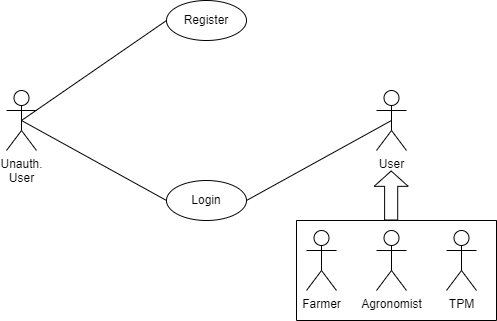
\includegraphics[scale=0.5]{/diagrams/RegistrationLoginUseCases.png}
			\caption{Registration and Login Use Case Diagram}
		\end{figure}
	
		\begin{figure}[h!]
			\centering
			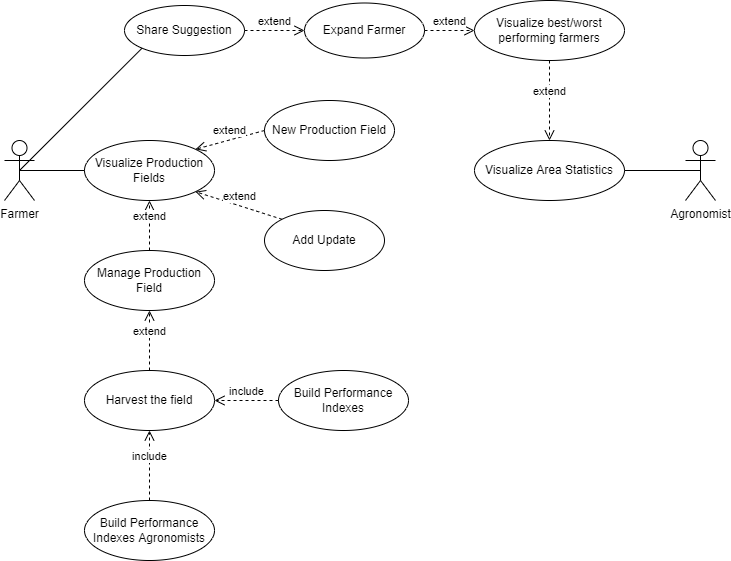
\includegraphics[scale=0.5]{/diagrams/FarmerAgronomistProductionArea.png}
			\caption{Production Area Use Case Diagram}
		\end{figure}
	
		\begin{figure}[h!]
		\centering
			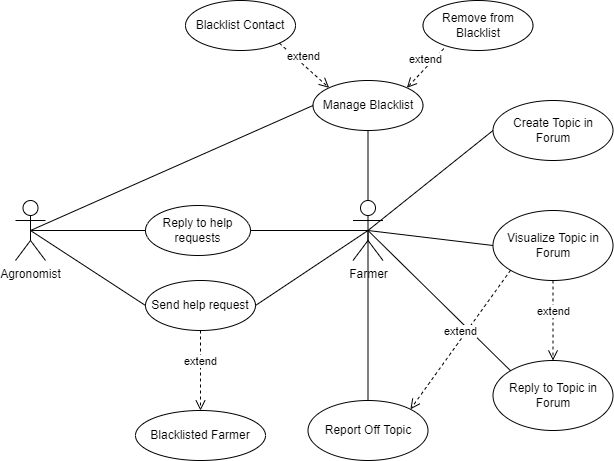
\includegraphics[scale=0.5]{/diagrams/FarmerCommunicationUseCases.png}
			\caption{Farmer Communication Use Case Diagram}
		\end{figure}
	
		\begin{figure}[h!]
			\centering
			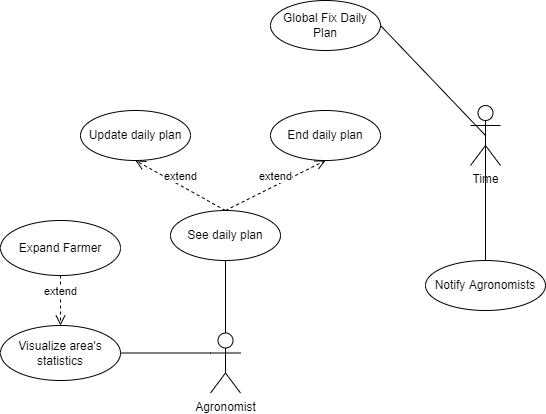
\includegraphics[scale=0.5]{/diagrams/AgronomistsDailyPlanFarmers.png}
			\caption{Agronomist Daily Plan Use Case Diagram}
		\end{figure}
	
		\begin{figure}[h!]
			\centering
			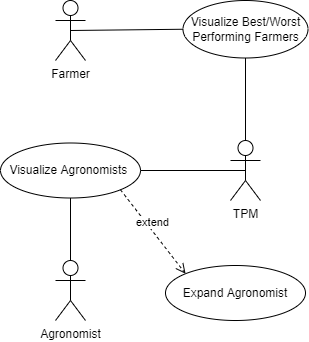
\includegraphics[scale=0.5]{/diagrams/TPMUseCases.png}
			\caption{TPM Use Case Diagram}
		\end{figure}
			
		\FloatBarrier
	
	\subsubsection[Use Cases Description]{\hyperlink{toc}{Use Cases Description}}
		\label{sec:useCases}
		
		\begin{enumerate}
			\item \textbf{Registration} 
				\begin{longtable}{p{0.26\linewidth}p{0.75\linewidth}}
					\toprule
					\textbf{Name} & \textbf{Registration} \\
					\midrule
					\textbf{Actors} & Unauth. User \\
					\midrule
					\textbf{Entry conditions} & The web application has started \\
					\midrule
					\textbf{Flow of events} & 
					\begin{enumerate}
						\item Unauth. User selects the "Register" option
						\item The system asks the type of registration ("Farmer", "Agronomist", "Telangana Policy Maker")
						\item Alternative flow A)
						\begin{enumerate}
							\item Unauth. User selects "Agronomist"
							\item The system asks for a valid Agronomist License
							\item Unauth. User uploads his license
							\item The system checks if the license is valid
							\item The system display the map of Telangana
							\item Unauth. User inserts his area of interest
						\end{enumerate}
						\item Alternative Flow B)
						\begin{enumerate}
							\item Unauth. User selects "Telangana Policy Maker"
							\item The system asks for a valid Telangana Policy Maker License
							\item Unauth. User uploads his license
							\item The system checks if the license is valid
						\end{enumerate}
						\item Alternative Flow C)
						\begin{enumerate}
							\item Unauth. User selects "Farmer"
							\item The system display the map of Telangana
							\item Unauth. User inserts his location
						\end{enumerate}
						\item The system displays mandatory registration fields(i.e: name,password,foto...) useful for the creation of the new User
						\item Unauth. User fills the mandatory fields and selects "Sign Up"
						\item The system preprocesses input data and stores it into the database
					\end{enumerate} \\
					\midrule
					\textbf{Exit conditions} & Unauth. User has now an User account and the User account contains valid data into the database according to its role.\\
					\midrule
					\textbf{Exceptions} & 
					\begin{itemize}
						\item If an existing user with the same credentials exist, the system displays an error message to Unauth. User
						\item If the preprocessed data in step 6 is not valid,  an error message is displayed to 
						Unauth. User
						\item If the GPS Area Mapping system fails, an error message is displayed to Unauth. User
						\item If the License is not valid, an error message is displayed to Unauth. User
					\end{itemize} \\
					\bottomrule
					\caption{\emph{User Registration} use case description}
				\end{longtable}
			
				\begin{figure}[h]
					\centering
					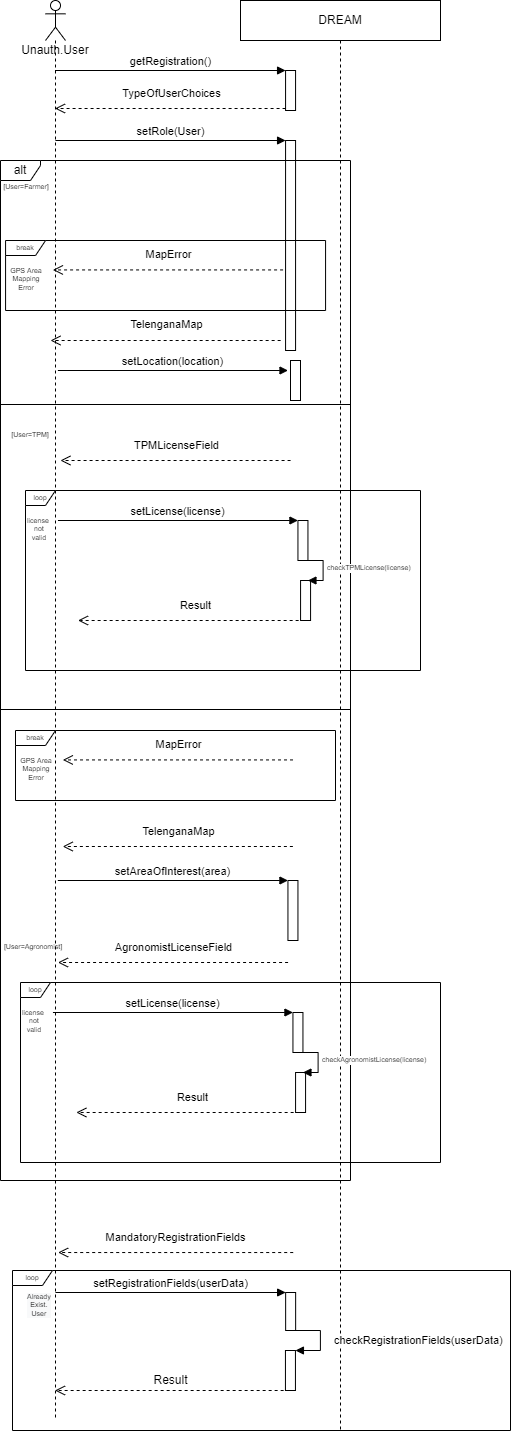
\includegraphics[scale=0.4]{/diagrams/sequences/Registration.png}
					\caption{User Registration sequence diagram}
				\end{figure}
				
				\FloatBarrier
			\item \textbf{User Login}
				\begin{longtable}{p{0.26\linewidth}p{0.75\linewidth}}
					\toprule
					\textbf{Name} & \textbf{User Login} \\
					\midrule
					\textbf{Actors} & Unauth. User, User \\
					\midrule
					\textbf{Entry conditions} & The web application has started \\
					\midrule
					\textbf{Flow of events} & 
					\begin{enumerate}
						\item Unauth. User selects the "Login" option
						\item The system displays mandatory fields useful for the authentication of the Unauth. User
						\item Unauth. User fills the fields and selects "Sign in"
						\item The system checks the existence of such User
						\item The system autenticates Unauth. User as User with his specific role
					\end{enumerate} \\
					\midrule
					\textbf{Exit conditions} &  Unauth. User has been autenticated as User and can proceed with the navigation in his homepage\\
					\midrule
					\textbf{Exceptions} & 
					\begin{itemize}
						\item  At any moment, the Unauth. User can stop the use case
						\item If the User does not exists, the system displays an error message		
					\end{itemize} \\
					\bottomrule
					\caption{\emph{User Login} use case description}
				\end{longtable}
			
				\begin{figure}[h]
					\centering
					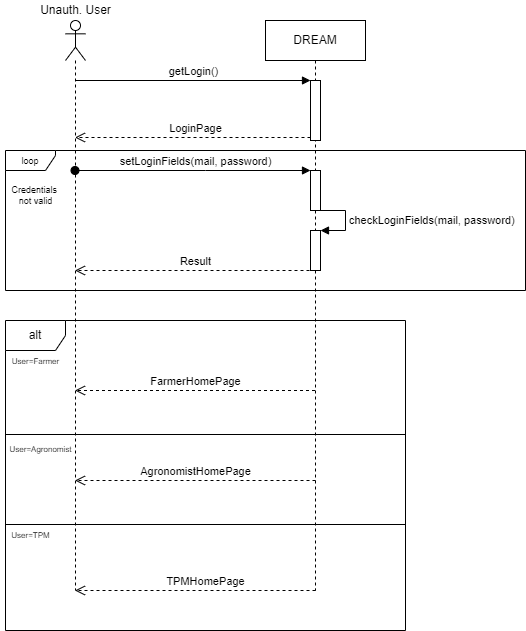
\includegraphics[scale=0.30]{/diagrams/sequences/Login.png}
					\caption{User Login sequence diagram}
				\end{figure}
			
				\FloatBarrier
				\newpage
			\item \textbf{New Production Field}
				\begin{longtable}{p{0.26\linewidth}p{0.75\linewidth}}
					\toprule
					\textbf{Name} & \textbf{New Production Field} \\
					\midrule
					\textbf{Actors} & Farmer \\
					\midrule
					\textbf{Entry conditions} & \begin{enumerate}
													\item Farmer is logged in the application
													\item Farmer visualizes the Home Page page
												\end{enumerate} \\
					\midrule
					\textbf{Flow of events} & 
					\begin{enumerate}
						\item Farmer selects "Insert" in Production window
						\item The system displays mandatory fields to specify the type of production 
						\item Farmer types production data into mandatory fields and presses "Confirm"
						\item The system preprocesses input data and stores it into the database
					\end{enumerate} \\
					\midrule
					\textbf{Exit conditions} & The new production field is correctly stored\\
					\midrule
					\textbf{Exceptions} & 
					\begin{itemize}
						\item Invalid Production Data Exception
					\end{itemize} \\
					\bottomrule
					\caption{\emph{Add Production Field} use case description}
				\end{longtable}
			
				\begin{figure}[h]
					\centering 
					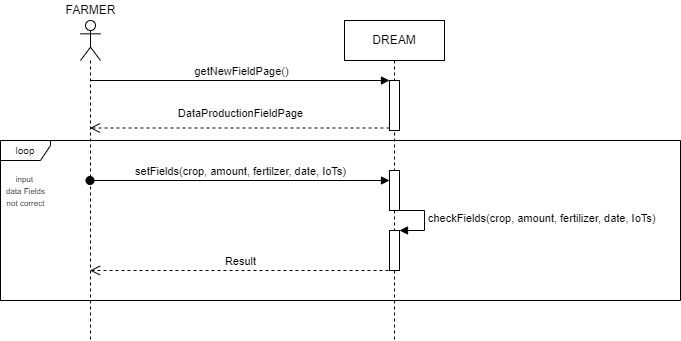
\includegraphics[scale=0.5]{/diagrams/sequences/Insert Data Production Fields.png}
					\caption{Insert Data Production Field sequence diagram}
				\end{figure}
			
				\FloatBarrier
				\newpage
			\item \textbf{Manage Production Field}
				\begin{longtable}{p{0.26\linewidth}p{0.75\linewidth}}
					\toprule
					\textbf{Name} & \textbf{Manage Production Field} \\
					\midrule
					\textbf{Actors} & Farmer \\
					\midrule
					\textbf{Entry conditions} & \begin{enumerate}
													\item Farmer must be authenticated
													\item Farmer is visualizing his production fields
												\end{enumerate}\\
					\midrule
					\textbf{Flow of events} & 
					\begin{enumerate}
						\item Farmer selects a production field
						\item The system expands the production field and the relative options
						\item Alternative Flow A)
						\begin{enumerate}
							\item Farmer selects "Edit Production Field"
							\item The system let Farmer to edit the production field editable data (i.e. planted crops, type, fertilizer..)
							\item Farmer confirms the edit
							\item The system stores the modified production field in the database
						\end{enumerate}
						\item Alternative Flow B)
						\begin{enumerate}
							\item Farmer selects "Remove Production Field"
							\item The system asks the farmer if the decision should be taken
							\item Farmer confirms the decision
							\item The system removes the production field from the database
						\end{enumerate}
					\end{enumerate} \\
					\midrule
					\textbf{Exit conditions} & All the production fields have been managed \\
					\midrule
					\textbf{Exceptions} & 
					\begin{itemize}
						\item Invalid Production Data Exception
					\end{itemize} \\
					\bottomrule
					\caption{\emph{Manage Production Field} use case description}
				\end{longtable}
			
				\begin{figure}[h]
					\centering
					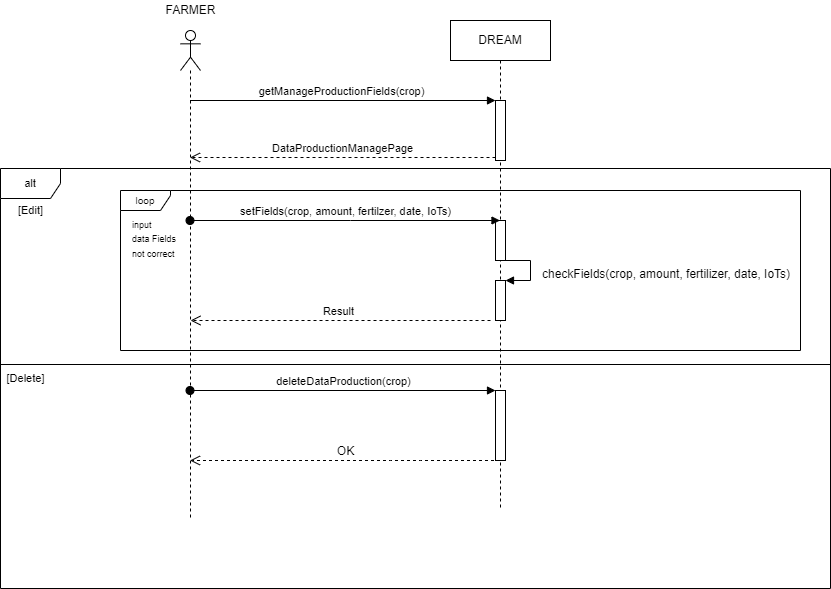
\includegraphics[scale=0.5]{/diagrams/sequences/ManageProductionField.png}
					\caption{Manage Production Field sequence diagram}
				\end{figure}
			
				\FloatBarrier
				\newpage
			\item \textbf{Add Update}
				\begin{longtable}{p{0.26\linewidth}p{0.75\linewidth}}
					\toprule
					\textbf{Name} & \textbf{Add Update} \\
					\midrule
					\textbf{Actors} & Farmer \\
					\midrule
					\textbf{Entry conditions} & \begin{enumerate}
													\item Farmer must be authenticated
													\item Farmer is in the Home Page page
												\end{enumerate} \\
					\midrule
					\textbf{Flow of events} & 
					\begin{enumerate}
						\item Farmer selects "Add Update" option
						\item The system displays fields to be filled to describe the problem/update or to insert a photo about that production field
						\item Farmer fills the fields
						\item Farmer presses "Confirm"
						\item The system stores the problem/update in the database and binds it with the selected production field
					\end{enumerate} \\
					\midrule
					\textbf{Exit conditions} & The update is correctly stored and bounded with the production field\\
					\midrule
					\textbf{Exceptions} & 
					\begin{itemize}
						\item Format Photo errore exception	
					\end{itemize} \\
					\bottomrule
					\caption{\emph{Add Update} use case description}
				\end{longtable}
			
				\begin{figure}[h]
					\centering
					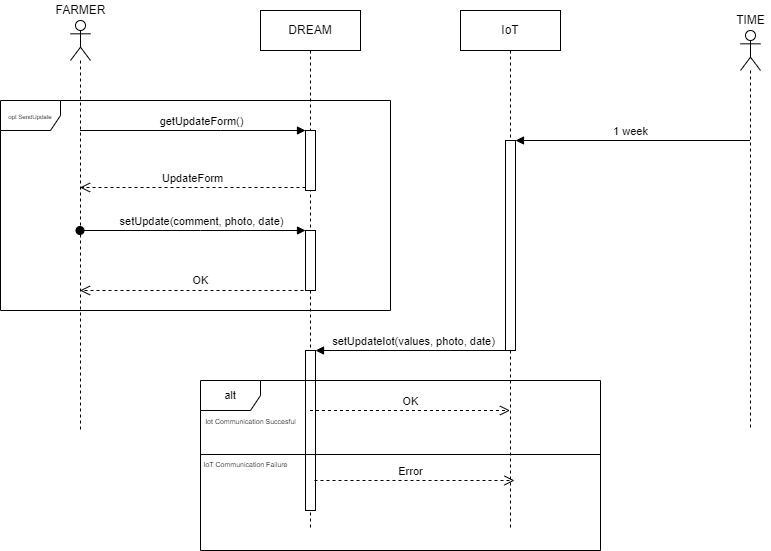
\includegraphics[scale=0.4]{/diagrams/sequences/AddUpdate.png}
					\caption{Add Update sequence diagram}
				\end{figure}
			
				\FloatBarrier
				\newpage
			\item \textbf{Harvest the field}
				\begin{longtable}{p{0.26\linewidth}p{0.75\linewidth}}
					\toprule
					\textbf{Name} & \textbf{Harvest the field} \\
					\midrule
					\textbf{Actors} & Farmer \\
					\midrule
					\textbf{Entry conditions} & \begin{itemize}
													\item Farmer must be authenticated
													\item Farmer is visualizing his production fields
													\item Farmer is in the Visualize Relevant Data page
												\end{itemize} \\
					\midrule
					\textbf{Flow of events} & 
					\begin{enumerate}
						\item Farmer selects "Harvest the field" option
						\item The system asks the amount of crops harvested and the ending data
						\item Farmer fills the field with a number
						\item Farmer selects "Confirm"
						\item The system removes the production field
						\item The system stores the above mentioned popped information in the database and uses them to update the statistics
					\end{enumerate} \\
					\midrule
					\textbf{Exit conditions} &  The production field is removed now. Statistics have been updated according to the pair (crop planted, crops harvested)\\
					\midrule
					\textbf{Exceptions} &  Format value inserted not accepted\\
					\bottomrule
					\caption{\emph{Harvest the field} use case description}
				\end{longtable}
			
			\item \textbf{Build Performance Indexes}
				\begin{longtable}{p{0.26\linewidth}p{0.75\linewidth}}
					\toprule
					\textbf{Name} & \textbf{Build Performance Indexes} \\
					\midrule
					\textbf{Actors} & Farmer \\
					\midrule
					\textbf{Entry conditions} & \begin{itemize}
													\item Farmer is logged in the application
												\end{itemize} \\
					\midrule
					\textbf{Flow of events} & 
					\begin{enumerate}
						\item The Farmer starts the use case when he harvests a production field
						\item The system then builds and updates statistics and performance indexes about the Farmer and the updated Production Field
					\end{enumerate} \\
					\midrule
					\textbf{Exit conditions} & New statistics are built according to the harvested production\\
					\midrule
					\textbf{Exceptions} &  \\
					\bottomrule
					\caption{\emph{Build Performance Indexes} use case description}
				\end{longtable}
			
				\begin{figure}[hbtp]
					\centering
					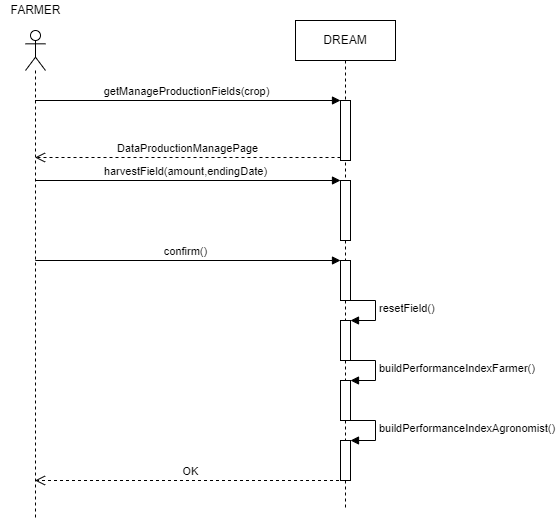
\includegraphics[scale=0.5]{/diagrams/sequences/HarvestField.png}
					\caption{Harvest field sequence diagram}
				\end{figure}
			
				\FloatBarrier
				\newpage
			\item \textbf{Send help request}
				\begin{longtable}{p{0.26\linewidth}p{0.75\linewidth}}
					\toprule
					\textbf{Name} & \textbf{Send help request} \\
					\midrule
					\textbf{Actors} & Farmer A, Farmer B, Agronomist \\
					\midrule
					\textbf{Entry conditions} & Farmer A is logged in the application \\
					\midrule
					\textbf{Flow of events} & 
					\begin{enumerate}
						\item Farmer A selects "Send help request" on his homepage
						\item The system displays email-like mandatory fields
						\item Farmer A inputs a description about the help he needs
						\item Farmer A specifies other mandatory fields 
						\item Farmer A specifies in particular the username of the Farmer A/Agronomist he wants to contact privately
						\item Farmer A presses "Send"
						\item The system stores the private message in the database and forwards a notification to the addressee
					\end{enumerate} \\
					\midrule
					\textbf{Exit conditions} & The inbox of the contacted Farmer B/Agronomist contains now the help request coming from the Farmer A\\
					\midrule
					\textbf{Exceptions} & 
					\begin{itemize}
						\item Blacklisted Farmer Exception in step f)
						\item Inexistent Contact Exception in step f) --> The addressee does not exists. The system displays an error message.
					\end{itemize} \\
					\bottomrule
					\caption{\emph{Send help request} use case description}
				\end{longtable}
	
	        \item \textbf{Blacklisted Farmer}
	        	\begin{longtable}{p{0.26\linewidth}p{0.75\linewidth}}
	        		\toprule
	        		\textbf{Name} & \textbf{Blacklisted Farmer} \\
	        		\midrule
	        		\textbf{Actors} & Farmer A, Farmer B, Agronomist \\
	        		\midrule
	        		\textbf{Entry conditions} & \begin{itemize}
	        										\item Farmer A is logged in the application
	        										\item Farmer A just pressed "Send" button to send help request to Farmer B/Agronomist
        										\end{itemize} \\
	        		\midrule
	        		\textbf{Flow of events} & 
	        		\begin{enumerate}
	        			\item Farmer is blacklisted by the addressee Farmer B/Agronomist
	        			\item The system displays an error message and a warning to Farmer A, inviting him to stop spamming
	        		\end{enumerate} \\
		        	\midrule
		        	\textbf{Exit conditions} & \\
		        	\midrule
		        	\textbf{Exceptions} &  \\
	        		\bottomrule
	        		\caption{\emph{Blacklisted Farmer} use case description}
	        	\end{longtable}
    	   
		
		\begin{figure}[h!]
			\centering
			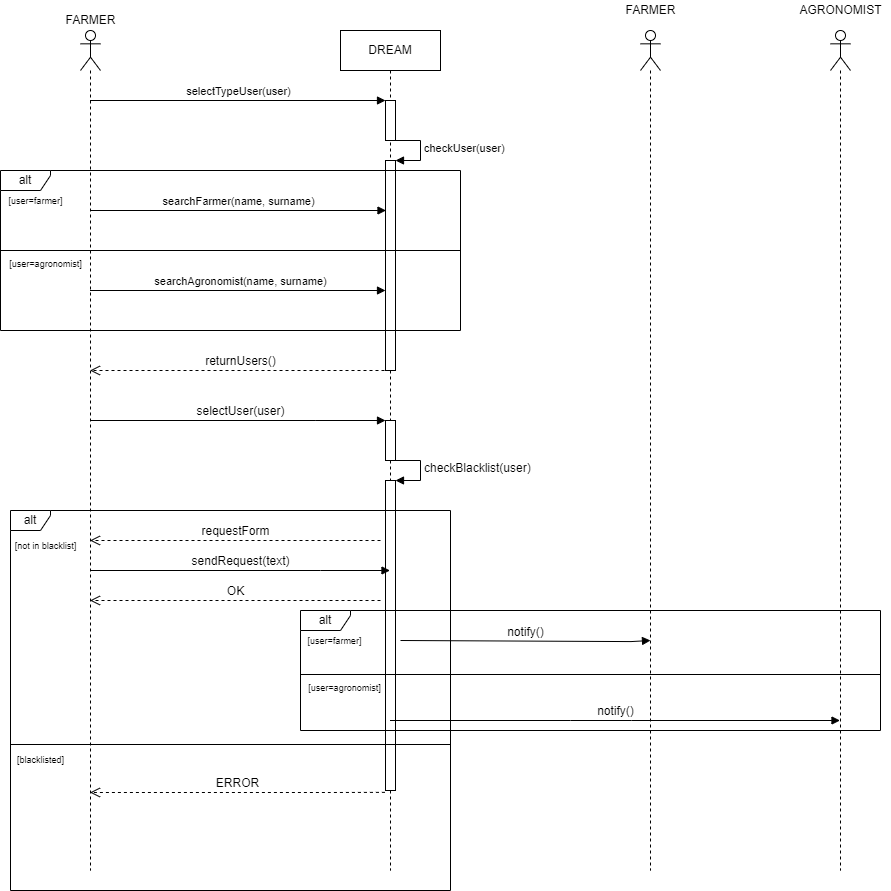
\includegraphics[scale=0.40]{/diagrams/sequences/SendRequest.png}
			\caption{Send Request sequence diagram}
		\end{figure}
			
		\FloatBarrier
		\newpage
		
	
			\item \textbf{Reply to help requests}
				\begin{longtable}{p{0.26\linewidth}p{0.75\linewidth}}
					\toprule
					\textbf{Name} & \textbf{Reply to help requests} \\
					\midrule
					\textbf{Actors} & Farmer A, Agronomist, Farmer B \\
					\midrule
					\textbf{Entry conditions} & Farmer A/Agronomist is logged in the application \\
					\midrule
					\textbf{Flow of events} & 
					\begin{enumerate}
						\item Farmer A/Agronomist selects "Check help requests" on his homepage
						\item The system lists all help requests for that Farmer A/Agronomist
						\item Farmer A/Agronomist selects one among them
						\item The system displays the content
						\item Farmer A/Agronomist selects "Reply"
						\item The system shows email-like mandatory fields
						\item Farmer A/Agronomist inputs data and the reply to the help request
						\item Farmer A presses "Send"
						\item The system stores in the database the reply
					\end{enumerate} \\
					\midrule
					\textbf{Exit conditions} & The inbox of the contacted Farmer B contains now the reply to his help request
					\\
					\midrule
					\textbf{Exceptions} & \\
					\bottomrule
					\caption{\emph{Reply to help requests} use case description}
				\end{longtable}
			
				\begin{figure}[h]
					\centering
					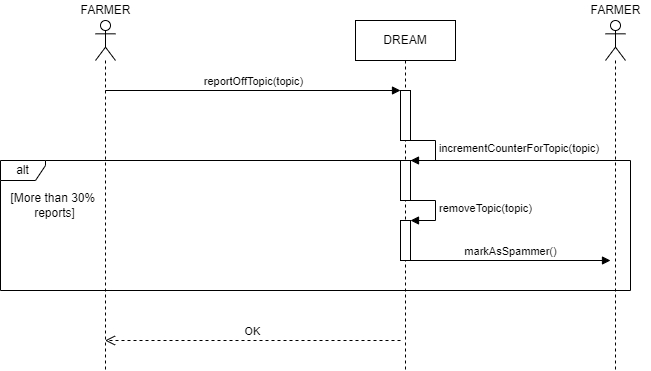
\includegraphics[scale=0.5]{/diagrams/sequences/ReplyToHelpRequest.png}
					\caption{Reply to help requests sequence diagram}
				\end{figure}
			
				\FloatBarrier
			\item \textbf{Blacklist Contact}
				\begin{longtable}{p{0.26\linewidth}p{0.75\linewidth}}
					\toprule
					\textbf{Name} & \textbf{Blacklist Contact} \\
					\midrule
					\textbf{Actors} & Farmer, Agronomist\\
					\midrule
					\textbf{Entry conditions} & \begin{itemize}
													\item Farmer/Agronomist is logged in the application
													\item Farmer/Agronomist visualizes his blacklist
												\end{itemize} \\
					\midrule
					\textbf{Flow of events} & 
					\begin{enumerate}
						\item Farmer/Agronomist inputs the name/surname of a contact in the search
						\item The system displays the list of retrieved contacts
						\item Farmer/Agronomist selects a contact
						\item Farmer/Agronomist presses the button "Add"
						\item The system stores the choice on the database and marks the selected contact as blacklisted for the Farmer/Agronomist
					\end{enumerate} \\
					\midrule
					\textbf{Exit conditions} & The selected contact is blacklisted\\
					\midrule
					\textbf{Exceptions} & \\
					\bottomrule
					\caption{\emph{Blacklist Contact} use case description}
				\end{longtable}
			
			\item \textbf{Remove from Blacklist}
				\begin{longtable}{p{0.26\linewidth}p{0.75\linewidth}}
					\toprule
					\textbf{Name} & \textbf{Remove from Blacklist} \\
					\midrule
					\textbf{Actors} & Farmer, Agronomist \\
					\midrule
					\textbf{Entry conditions} & \begin{itemize}
													\item Farmer/Agronomist is logged in the application
													\item Farmer/Agronomist visualizes his blacklist
												\end{itemize} \\
					\midrule
					\textbf{Flow of events} & 
					\begin{enumerate}
						\item Farmer/Agronomist expanded a contact in the Blacklist page
						\item Farmer selected "Remove Contact"
						\item The system stores the choice on the database and unmarks the blacklisted user
					\end{enumerate} \\
					\midrule
					\textbf{Exit conditions} & The list is shown to the authority\\
					\midrule
					\textbf{Exceptions} &  The selected contact is no more in the blacklist\\
					\bottomrule
					\caption{\emph{Check unread reports} use case description}
				\end{longtable}
				
				\begin{figure}[h]
					\centering
					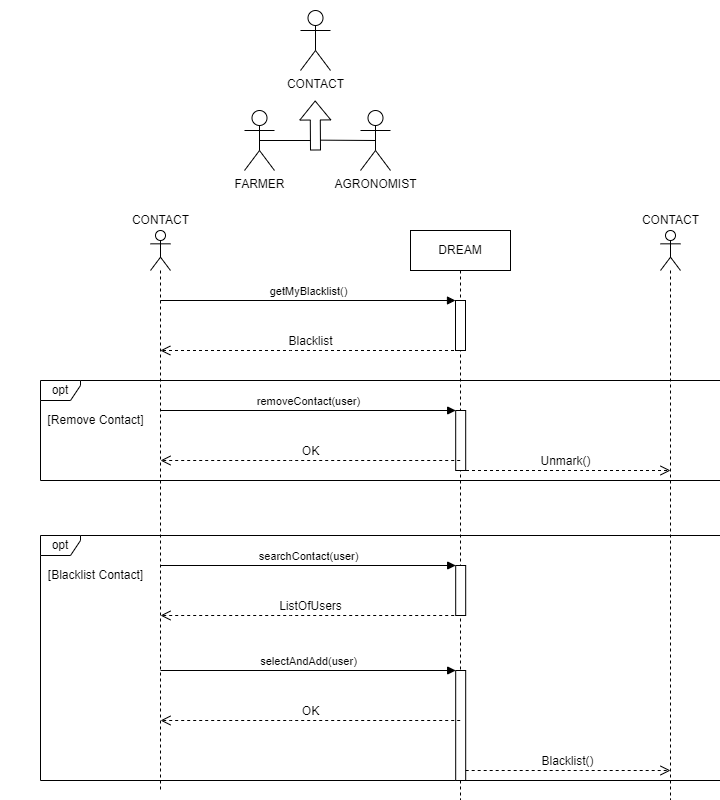
\includegraphics[scale=0.5]{/diagrams/sequences/ManageBlacklist.png}
					\caption{Manage Blacklist sequence diagram}
				\end{figure}
				
				\FloatBarrier
				\newpage
			\item \textbf{Create Topic in Forum}
				\begin{longtable}{p{0.26\linewidth}p{0.75\linewidth}}
					\toprule
					\textbf{Name} & \textbf{Create Topic in Forum} \\
					\midrule
					\textbf{Actors} & Farmer\\
					\midrule
					\textbf{Entry conditions} & Farmer is logged in the application \\
					\midrule
					\textbf{Flow of events} & 
					\begin{enumerate}
						\item Farmer selects "Forum" on his homepage
						\item The system displays mandatory fields about the type of discussion forum to be created
						\item Farmer specifies all the information and inserts a first post
						\item Farmer presses "Create"
						\item The system checks if the last topic created by the farmer is not up to the current day
						\item The system creates the discussion forum and stores it into the database
					\end{enumerate} \\
					\midrule
					\textbf{Exit conditions} & The new Topic is visible now\\
					\midrule
					\textbf{Exceptions} &  
					\begin{enumerate}
						\item Daily Topics Limit Reached Exception in e) --> Only one topic per day is allowed, so the daily topics limit has been reached by the current farmer; an error message is displayed and the use case stops
					\end{enumerate}\\
					\bottomrule
					\caption{\emph{Create Topic in Forum} use case description}
				\end{longtable}
	
				\begin{figure}[hbtp]
					\centering
					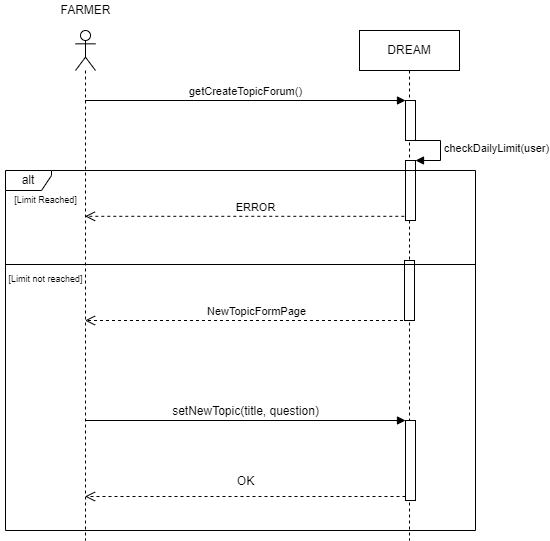
\includegraphics[scale=0.45]{/diagrams/sequences/CreateDiscussionForum.png}
					\caption{Create Topic in Forum sequence diagram}
				\end{figure}
			
				\FloatBarrier
				\newpage
		
			\item \textbf{Visualize Topic in Forum}
				\begin{longtable}{p{0.26\linewidth}p{0.75\linewidth}}
					\toprule
					\textbf{Name} & \textbf{Visualize Topic in Forum} \\
					\midrule
					\textbf{Actors} & Farmer\\
					\midrule
					\textbf{Entry conditions} & Farmer is logged in the application \\
					\midrule
					\textbf{Flow of events} & 
					\begin{enumerate}
						\item Farmer selects "Forum" on his homepage
						\item The system displays the lists of topics sorted in chronological order
						\item Farmer selects a topic
						\item The system displays the comments of that topic
					\end{enumerate} \\
					\midrule
					\textbf{Exit conditions} & The topic selected with all comments is visible now\\
					\midrule
					\textbf{Exceptions} &  \\
					\bottomrule
					\caption{\emph{Visualize Topic in Forum} use case description}
				\end{longtable}
			
			\item \textbf{Reply to topic in Forum}
				\begin{longtable}{p{0.26\linewidth}p{0.75\linewidth}}
					\toprule
					\textbf{Name} & \textbf{Reply to topic in Forum} \\
					\midrule
					\textbf{Actors} & Farmer\\
					\midrule
					\textbf{Entry conditions} & \begin{enumerate}
													\item Farmer is logged in the application
													\item Farmer visualizes a topic
												\end{enumerate} \\
					\midrule
					\textbf{Flow of events} & 
					\begin{enumerate}
						\item Farmer selects "Reply"
						\item The system displays a field for the reply
						\item Farmer inputs the reply and presses "Send"
						\item The system stores the reply in the database and appends it to the conversation
					\end{enumerate} \\
					\midrule
					\textbf{Exit conditions} & Farmer's reply is shown in the topic \\
					\midrule
					\textbf{Exceptions} &  \\
					\bottomrule
					\caption{\emph{Reply to topic in Forum} use case description}
				\end{longtable}
		
				\begin{figure}[hbtp]
					\centering
					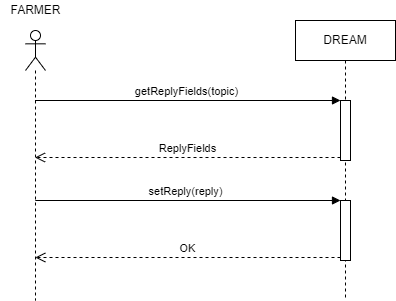
\includegraphics[scale=0.45]{/diagrams/sequences/ReplyToDiscussionForum.png}
					\caption{Create Topic in Forum sequence diagram}
				\end{figure}
			
				\FloatBarrier
			
			\item \textbf{Report Off topic}
				\begin{longtable}{p{0.26\linewidth}p{0.75\linewidth}}
					\toprule
					\textbf{Name} & \textbf{Report Off topic} \\
					\midrule
					\textbf{Actors} & Farmer A, Farmer B \\
					\midrule
					\textbf{Entry conditions} & \begin{enumerate}
													\item Farmer A is logged in the application
													\item Farmer A visualizes a discussion forum
													\item Another Farmer (Farmer B) goes off topic
												\end{enumerate} \\
					\midrule
					\textbf{Flow of events} & 
					\begin{enumerate}
						\item Farmer A selects "Report Off Topic" for a specific post of Farmer B
						\item The system stores the report in the database
						\item The system counts how many reports for that specific post/Farmer B have been sent
						\item Alternative Flow B)
						\begin{enumerate}
							\item The system counts more than 30 percent of active farmers reports for the post
							\item The system removes the off topic post and marks Farmer B as "Spammer" for that forum
						\end{enumerate}
					\end{enumerate} \\
					\midrule
					\textbf{Exit conditions} & Farmer A has succefully reported Farmer B's off topic post and Farmer B's off topic post is correctly managed by the system \\
					\midrule
					\textbf{Exceptions} &  \\
					\bottomrule
					\caption{\emph{Report Off topic} use case description}
				\end{longtable}
			
				\begin{figure}[hbtp]
					\centering
					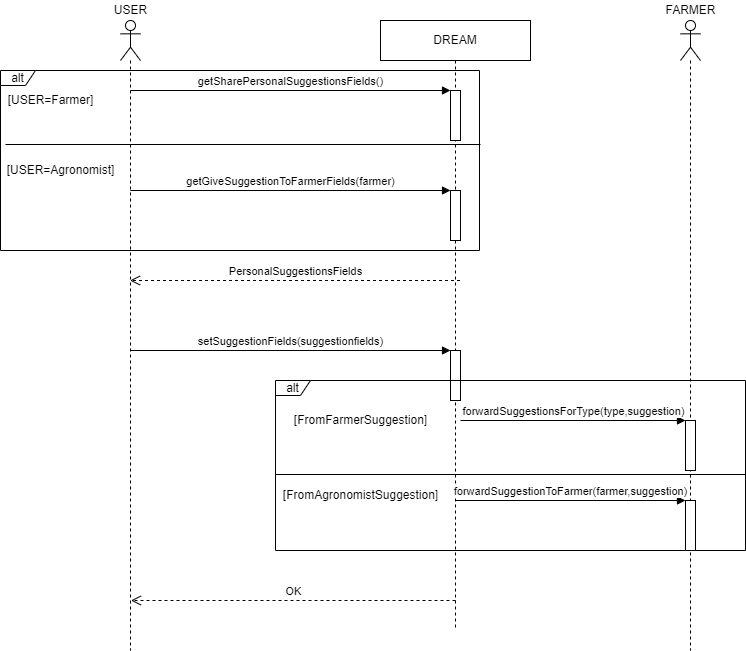
\includegraphics[scale=0.45]{/diagrams/sequences/ReportOffTopic.png}
					\caption{Report Off topic sequence diagram}
				\end{figure}
			
			\item \textbf{See daily plan}
				\begin{longtable}{p{0.26\linewidth}p{0.75\linewidth}}
					\toprule
					\textbf{Name} & \textbf{See daily plan} \\
					\midrule
					\textbf{Actors} & Agronomist \\
					\midrule
					\textbf{Entry conditions} &	Agronomist is logged in the application\\
					\midrule
					\textbf{Flow of events} & 
					\begin{enumerate}
						\item Farmer selects "See daily plan" on his homepage
						\item The system displays the daily plan to the Agronomist.
					\end{enumerate} \\
					\midrule
					\textbf{Exit conditions} & The Agronomist is now able to see the daily plan\\
					\midrule
					\textbf{Exceptions} &  \\
					\bottomrule
					\caption{\emph{See daily plan} use case description}
				\end{longtable}
			
			\item \textbf{Fix daily plan}
				\begin{longtable}{p{0.26\linewidth}p{0.75\linewidth}}
					\toprule
					\textbf{Name} & \textbf{Fix daily plan} \\
					\midrule
					\textbf{Actors} & Time \\
					\midrule
					\textbf{Entry conditions} & \\
					\midrule
					\textbf{Flow of events} & 
					\begin{enumerate}
						\item Time starts the use case when it becomes 0.00 for the current day
						\item For all agronomists the system marks the daily plan which has a temporal window of a month as confirmed and makes it immutable
						\item For all agronomists the system creates a new daily plan for the next day
					\end{enumerate} \\
					\midrule
					\textbf{Exit conditions} & For all agronomists the daily plan is immutable now for each day a new daily plan is created. \\
					\midrule
					\textbf{Exceptions} &  \\
					\bottomrule
					\caption{\emph{Fix daily plan} use case description}
				\end{longtable}
			
			\item \textbf{Update daily plan}
				\begin{longtable}{p{0.26\linewidth}p{0.75\linewidth}}
					\toprule
					\textbf{Name} & \textbf{Update daily plan} \\
					\midrule
					\textbf{Actors} & Agronomist \\
					\midrule
					\textbf{Entry conditions} & \begin{enumerate}
						\item Agronomist is logged in the application
						\item Agronomist sees his daily plan in the application
						\item The daily plan is not fixed
					\end{enumerate} \\
					\midrule
					\textbf{Flow of events} & 
					\begin{enumerate}
						\item Alternative Flow A)
						\begin{enumerate}
							\item Agronomist selects "Add visit"
							\item The system displays editable fields (i.e farmer, hour) about the new visit
							\item Agronomist updates the fields and selects "Finish"
							\item The system stores the visit in the database
						\end{enumerate}
						\item Alternative Flow B)
						\begin{enumerate}
							\item Agronomist selects "Delete visit"
							\item Agronomist selects the visits to be deleted 
							\item Agronomist selects "Finish"
							\item The system deletes the visits in the database
						\end{enumerate}
					\end{enumerate} \\
					\midrule
					\textbf{Exit conditions} & The daily plan is updated in the database \\
					\midrule
					\textbf{Exceptions} &  \\
					\bottomrule
					\caption{\emph{Update daily plan} use case description}
				\end{longtable}
			
			\item \textbf{End daily plan}
				\begin{longtable}{p{0.26\linewidth}p{0.75\linewidth}}
					\toprule
					\textbf{Name} & \textbf{End daily plan} \\
					\midrule
					\textbf{Actors} & Agronomist, Time \\
					\midrule
					\textbf{Entry conditions} & \begin{enumerate}
						\item Agronomist is logged in the application
						\item Agronomist sees his daily plan in the application
						\item The daily plan is not fixed
					\end{enumerate} \\
					\midrule
					\textbf{Flow of events} & 
					\item Agronomist selects "Confirm daily plan"
					\item The system marks the daily plan as confirmed and makes it immutable \\
					\midrule
					\textbf{Exit conditions} & The daily plan is immutable now \\
					\midrule
					\textbf{Exceptions} &  \\
					\bottomrule
					\caption{\emph{Update daily plan} use case description}
				\end{longtable}
			
				\begin{figure}[hbtp]
					\centering
					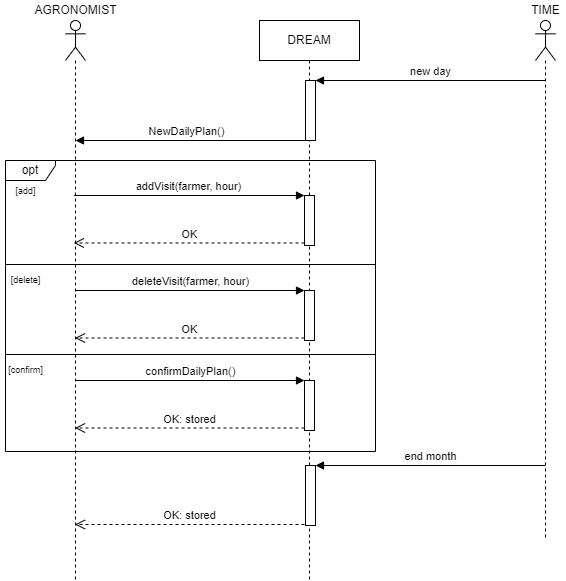
\includegraphics[scale=0.45]{/diagrams/sequences/ManageDailyPlan.png}
					\caption{Manage Daily Plan sequence diagram}
				\end{figure}
			
				\FloatBarrier
			
			\item \textbf{Notify Agronomists}
				\begin{longtable}{p{0.26\linewidth}p{0.75\linewidth}}
					\toprule
					\textbf{Name} & \textbf{Notify Agronomists} \\
					\midrule
					\textbf{Actors} & Time, Agronomist \\
					\midrule
					\textbf{Entry conditions} & \\
					\midrule
					\textbf{Flow of events} & 
					\begin{enumerate}
						\item Time starts the use case when it ends the last day of the current month
						\item The system retrieves all the farmers which has not been visited at least twice and their location
						\item The system retrieves all the agronomists related to the retrieved locations
						\item The system notifies the aforesaid agronomists about the previously retrieved farmers, as they need to be visited
					\end{enumerate} \\
					\midrule
					\textbf{Exit conditions} & All the agronomists have been notified \\
					\midrule
					\textbf{Exceptions} &  \\
					\bottomrule
					\caption{\emph{Notify Agronomists} use case description}
				\end{longtable}
			
				\begin{figure}[hbtp]
					\centering
					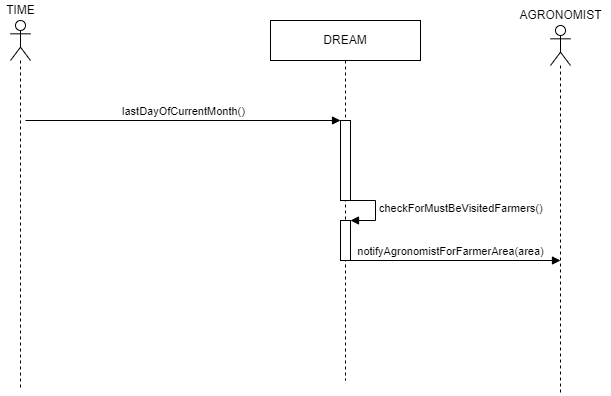
\includegraphics[scale=0.45]{/diagrams/sequences/NotifyAgronomists.png}
					\caption{Notify Agronomists sequence diagram}
				\end{figure}
			
			\item \textbf{Share Suggestion}
				\begin{longtable}{p{0.26\linewidth}p{0.75\linewidth}}
					\toprule
					\textbf{Name} & \textbf{Share Suggestion} \\
					\midrule
					\textbf{Actors} & Agronomist, Farmer A, Farmer B \\
					\midrule
					\textbf{Entry conditions} & \begin{enumerate}
						\item The appropriate user (which is one among Agronomist or Farmer A) is authenticated
						\item If Agronomist is authenticated then he has expanded Farmer B's view
					\end{enumerate} \\
					\midrule
					\textbf{Flow of events} & 
					\item Farmer A selects "Share Personal Suggestion"
					\item Alterantive Flow A)
					\begin{enumerate}
						\item Agronomist selects "Give Suggestion"
					\end{enumerate} 
					\item The system displays useful forms for the suggestion (e.g target type of production...) and a textarea
					\item Agronomist/Farmer A fills the textarea with useful suggestions about a particular production field or more general tips
					\item Agronomist/Farmer A selects "Publish Suggestion"
					\item The system stores in the database the suggestion
					\item For each Farmer B that owns a production field targeted by the suggestion based on specific parameters (type of production..) the system forwards to him the personalized suggestion
					\item Alternative flow A)
					\begin{enumerate}
						\item The system forwards to Farmer B (whose view was expanded by the Agronomist) the suggestion of the Agronomist
					\end{enumerate} \\
					\midrule
					\textbf{Exit conditions} & \begin{enumerate}
						\item Farmer A's suggestion is now forwarded and visible to all Farmer Bs that own a production field targeted by the suggestion
						\item Agronomist's suggestion is now forwarded and visible to the expanded Farmer B.
					\end{enumerate} \\
					\midrule
					\textbf{Exceptions} &  \\
					\bottomrule
					\caption{\emph{Share Suggestion} use case description}
				\end{longtable}
			
				\begin{figure}[hbtp]
					\centering
					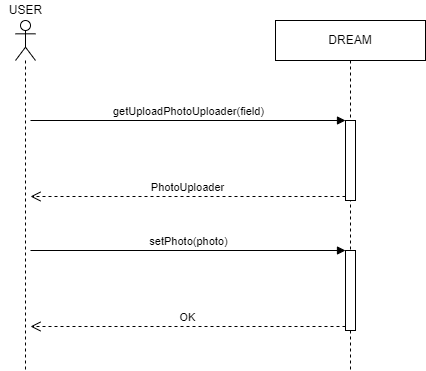
\includegraphics[scale=0.45]{/diagrams/sequences/ShareSuggestion.png}
					\caption{Share Suggestion sequence diagram}
				\end{figure}
			
			\FloatBarrier
			
			\item \textbf{Visualize Area Statistics}
				\begin{longtable}{p{0.26\linewidth}p{0.75\linewidth}}
					\toprule
					\textbf{Name} & \textbf{Visualize Area Statistics} \\
					\midrule
					\textbf{Actors} & Agronomist\\
					\midrule
					\textbf{Entry conditions} & \begin{enumerate}
						\item Agronomist is logged in the application
						\item The database contains the area of interest of the Agronomist
					\end{enumerate} \\
					\midrule
					\textbf{Flow of events} & 
					\item Agronomist selects "Visualize Area Statistics"
					\item The system displays all the area statistics to the Agronomist \\
					\midrule
					\textbf{Exit conditions} & Area Statistics now visible \\
					\midrule
					\textbf{Exceptions} &  \\
					\bottomrule
					\caption{\emph{Visualize Area Statistics} use case description}
				\end{longtable}
			
			\item \textbf{Visualize best/worst performing farmers}
				\begin{longtable}{p{0.26\linewidth}p{0.75\linewidth}}
					\toprule
					\textbf{Name} & \textbf{Visualize best/worst performing farmers} \\
					\midrule
					\textbf{Actors} & Agronomist,TPM \\
					\midrule
					\textbf{Entry conditions} & \begin{enumerate}
						\item The appropriate user (which is one among Agronomist or TPM) is authenticated
						\item If Agronomist is authenticated then he has selected his area of interest
					\end{enumerate} \\
					\midrule
					\textbf{Flow of events} & 
					\item TPM selects "Visualize best performing farmers"
					\item Alternative flow A)
					\begin{enumerate}
						\item Agronomist selects "Visualize best/worst performing farmers"
						\item The system restricts the displayable farmers to those working in the area of interested of the Agronomist
					\end{enumerate}
					\item The system displays the list of displayable farmers and their relative performances \\
					\midrule
					\textbf{Exit conditions} & Performance of the farmers are now visible \\
					\midrule
					\textbf{Exceptions} &  \\
					\bottomrule
					\caption{\emph{Visualize Area Statistics} use case description}
				\end{longtable}
				
			\begin{figure}[hbtp]
				\centering
				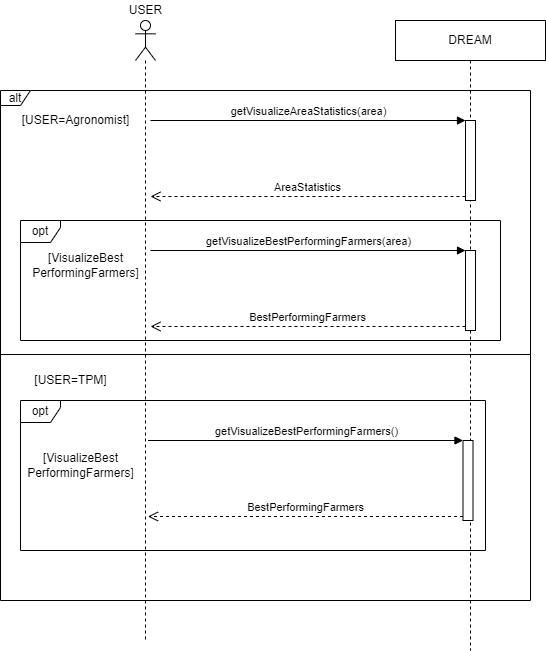
\includegraphics[scale=0.45]{/diagrams/sequences/Area_or_General_Statistics.png}
				\caption{Area of General Statistics sequence diagram}
			\end{figure}
		
		\FloatBarrier
					
			\item \textbf{Visualize Agronomists}
				\begin{longtable}{p{0.26\linewidth}p{0.75\linewidth}}
					\toprule
					\textbf{Name} & \textbf{Visualize Agronomists} \\
					\midrule
					\textbf{Actors} & Agronomist,TPM \\
					\midrule
					\textbf{Entry conditions} & TPM is authenticated \\
					\midrule
					\textbf{Flow of events} & 
					\item TPM selects "Visualize Agronomists"
					\item The system displays a list of agronomists and their working area \\
					\midrule
					\textbf{Exit conditions} & Agronomists are now visible \\
					\midrule
					\textbf{Exceptions} &  \\
					\bottomrule
					\caption{\emph{Visualize Agronomists} use case description}
				\end{longtable}
			
			\item \textbf{Visualize Relevant Data}
				\begin{longtable}{p{0.26\linewidth}p{0.75\linewidth}}
					\toprule
					\textbf{Name} & \textbf{Visualize Relevant Data} \\
					\midrule
					\textbf{Actors} & Farmer \\
					\midrule
					\textbf{Entry conditions} & \begin{enumerate}
						\item Farmer is logged in the application
						\item Farmer defined in the system his location and his production
						\item Farmer selected a field in "Manage Production Fields" page
					\end{enumerate} \\
					\midrule
					\textbf{Flow of events} & 
					\item Farmer selects "Visualize relevant data
					\item The system displays data relevant to the type of production based on the selected field
					\item The system displays weather forecasts
					\item The system displays personalized suggestions about the selected production \\
					\midrule
					\textbf{Exit conditions} & Data relevant to production fields are now visible \\
					\midrule
					\textbf{Exceptions} &  \\
					\bottomrule
					\caption{\emph{Visualize Relevant Data} use case description}
				\end{longtable}
			
			\item \textbf{Visualize Production Fields}
				\begin{longtable}{p{0.26\linewidth}p{0.75\linewidth}}
					\toprule
					\textbf{Name} & \textbf{Visualize Production Fields} \\
					\midrule
					\textbf{Actors} & Farmer \\
					\midrule
					\textbf{Entry conditions} & Farmer must be authenticated  \\
					\midrule
					\textbf{Flow of events} & 
					\item Farmer selects "Visualize Production Fields"
					\item The system displays all the production fields of the Farmer \\
					\midrule
					\textbf{Exit conditions} & The list of all production fields are now visible \\
					\midrule
					\textbf{Exceptions} &  \\
					\bottomrule
					\caption{\emph{Visualize Production Fields} use case description}
				\end{longtable}
			
			\item \textbf{Expand Agronomist}
				\begin{longtable}{p{0.26\linewidth}p{0.75\linewidth}}
					\toprule
					\textbf{Name} & \textbf{Expand Agronomist} \\
					\midrule
					\textbf{Actors} & TPM \\
					\midrule
					\textbf{Entry conditions} & \begin{enumerate}
						\item TPM is logged in the application
						\item TPM sees the "Visualize Agronomists" page
					\end{enumerate}  \\
					\midrule
					\textbf{Flow of events} & 
					\item TPM selects an agronomist among listed ones
					\item The system shows statistics and helped farmers for the selected agronomist \\
					\midrule
					\textbf{Exit conditions} & The data and the statistics relevant to an agronomist is now visible \\
					\midrule
					\textbf{Exceptions} &  \\
					\bottomrule
					\caption{\emph{Expand Agronomist} use case description}
				\end{longtable}
			
			\item \textbf{Expand Farmer}
				\begin{longtable}{p{0.26\linewidth}p{0.75\linewidth}}
					\toprule
					\textbf{Name} & \textbf{Expand Farmer} \\
					\midrule
					\textbf{Actors} & Agronomist \\
					\midrule
					\textbf{Entry conditions} & \begin{enumerate}
						\item Agronomist is logged in the application
						\item Agronomist sees the "Visualize Area's Statistics" page
					\end{enumerate}  \\
					\midrule
					\textbf{Flow of events} & 
					\item The Agronomist select a farmer among listed ones
					\item The system shows statistics about the selected farmer
					\item The system shows all the fields own by the selected farmer \\
					\midrule
					\textbf{Exit conditions} & All the statistics of the selected farmer are now visible \\
					\midrule
					\textbf{Exceptions} &  \\
					\bottomrule
					\caption{\emph{Expand Agronomist} use case description}
				\end{longtable}
				
				\begin{figure}[hbtp]
					\centering
					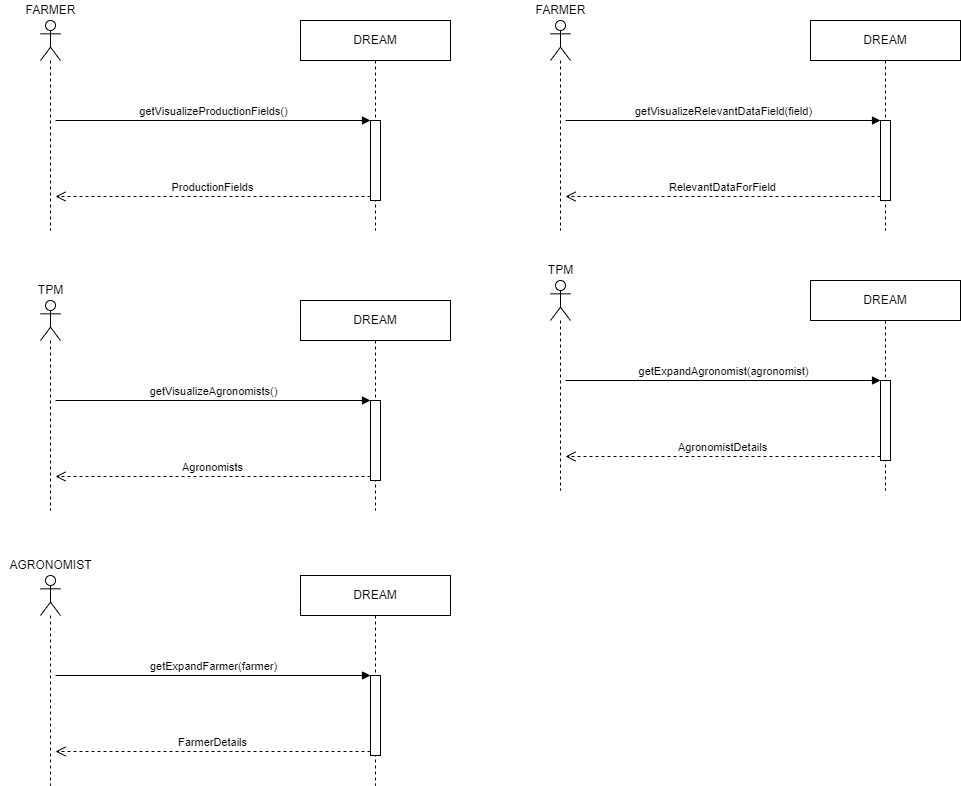
\includegraphics[scale=0.45]{/diagrams/sequences/OtherVisualizationSequences.png}
					\caption{Other Visualizations sequence diagram}
				\end{figure}
					
	\end{enumerate}

	\FloatBarrier
	\newpage
	
	\subsection[Performance Requirements]{\hyperlink{toc}{Performance Requirements}}
		\label{sec:performanceRequirements}
		
	\subsection[Product Requirments Usability]{\hyperlink{toc}{Product Requirments - Usability}}
	One of the main usability factors of DREAM is the ease of learning. As the application will be (potentially) used by old-school farmers and agronomists, their experience facing the features of the system should be easy and of simple use; it means: understandable functions and terminology, clear interpretation of graphs, etc.
	
	\subsection[Product Requirments Efficiency]{\hyperlink{toc}{Product Requirments - Efficiency}}
	As the application will support the interaction of three type of users who in turn can use simultaneously the application in a great number, DREAM must be able to manage the pool of incoming connections and reply to them properly. Since the system does not aim to solve critical (i.e. life or death) functions, it is more a matter of space rather than response  time. So, the system must be able to store a large quantity of data even for each user, as a Farmer is associated with graph(-s), production fields, discussion topics and inbox.
	
	
	\subsection[Design Constraints]{\hyperlink{toc}{Design Constraints}}
		\subsubsection[Standards Compliance]{\hyperlink{toc}{Standards Compliance}}
			\label{sec:standardCompliance}
			Formats: rainfall parameter in meteorological data is expressed in millimeters (mm).
			Agronomist and Telengana's Policy Maker licenses must be in pdf format and they must comply with standars for legal licenses. 
			Photos must be in png, jpg or bmp format. \\
			
			Legal Aspects: since DREAM supports personal data sharing, private and public messaging, its functions must be subject to the Harmful Digital Communication Act. Furthermore, privacy of data has to be guaranteed, so the system must follow the rules of the General Data Protection Regulations (GDPR).
		\subsubsection[Hardware Limitations]{\hyperlink{toc}{Hardware Limitations}}
			As specified in the Hardware Interface sections, the main hardware limitations are:
			
			\begin{enumerate}
				\item Connection to internet
				\item Properly working sensors for monitoring soil state and water irrigation (only if specified by the Farmer)
				\item Properly working cameras in sensors for taking photos of the field or a device able to take pictures (only if specified by the Farmer)
			\end{enumerate}
		
		\subsubsection[Any other Constraint]{\hyperlink{toc}{Any other Constraint}}
			Discussion Forums Constraints: a Farmer is limited to only 1 topic a day. A topic that receives off-topic reports from the 30 percent or more of active farmers in the discussion forum will be removed. \\
			
			Inbox Constraints: inbox of Farmer and Agronomist can contain 100 requests max received or sent. \\
			
			Production Fields Constraints: a Farmer is limited to 30 Production Fields.
	
	\subsection[Software System Attributes]{\hyperlink{toc}{Software System Attributes}}
		\subsubsection[Reliability]{\hyperlink{toc}{Reliability}}
		A crucial aspect of DREAM is the reliable store of important data. A Farmer should not met the risk of losing data about his production field, as it will damage him (who trusts DREAM) and Agronomists who choose to help him (who see unconsistent data and then elaborate inefficient strategies); Telengana's Policy Makers too can be affected by the problem, as the performance indexes built on missing/erroneous data of a Farmer can lead to misreadings/misunderstandings of the above mentioned actors. To avoid this risks, fault tolerance should be the main reliable requiremet of DREAM, and can be ensured by redundant data (for example by implementing RAID 4 disks with parity bit to retrieve lost data) and reducing to minimum the MTTDL.
		\subsubsection[Availability]{\hyperlink{toc}{Availability}}
		As mentioned in the Efficiency section, DREAM does not need critical response times or so, however it has to ensure that no one of the simultaneously connected users/sessions will suffer of starvation, hence every istance currently connected to the system should be equally served with a proper response time.
		\subsubsection[Security]{\hyperlink{toc}{Security}}
		DREAM functionalities are about storing sensitive informations about the user itself and (in the case of the Farmer) his production. As privacy is an important aspect of the system, the database must be able to implement access control methods to avoid unauthorized users to extract private informations. Since DREAM runs on browser, countermeasures againsts XSS and SQL injections attacks must be taken; this means implement prepared statementes whenever a query is called, preprocess all the input data to avoid Stored XSS, Reflected XSS and DOM XSS; cross-site-reforgery-tokens must be implemented whenever POST request are triggered (i.e. on update/creation of production fields, or on sending private messages). Sessions and data sent by the user must be encrypted with SHA-256 or better. Last but not least, the site has to own a valid and up do date SSL Certificate.
		
		\subsubsection[Maintainability]{\hyperlink{toc}{Maintainability}}
		The system must be developed in a way that future maintenance operations can be performed in an easy way. This means: clear and understandable bounds among components and tiers, well commented code, reuse of code.
		\subsubsection[Portability]{\hyperlink{toc}{Portability}}
		DREAM runs on browsers, so the most important web engines like Internet Explorer, Chrome, Firefox, Safari, Opera, and others must be able to render pages in a common or, if not, understandable fashion. If the website is accessed by Android browsers, the user must be able to see them in a resized and proper way
		
		\subsubsection[Scalability]{\hyperlink{toc}{Scalability}}
		As mentioned before, DREAM must be able to offer a connection pool and a storing space to a large quantity of users for three different type of actors.
	
		\FloatBarrier
		\newpage